% Chapter results

\chapter{Results} % Main chapter title

\label{Chapter3} % For referencing the chapter elsewhere, use \ref{Chapter3} 

%----------------------------------------------------------------------------------------

% Define some commands to keep the formatting separated from the content 
\newcommand{\keyword}[1]{\textbf{#1}}
\newcommand{\tabhead}[1]{\textbf{#1}}
\newcommand{\code}[1]{\texttt{#1}}
\newcommand{\file}[1]{\texttt{\bfseries#1}}
\newcommand{\option}[1]{\texttt{\itshape#1}}

%~~~~~~~~~~~~~~~~~~~~~~~~~~~~~~~~~~~~~~~~~~~~~~~~~~~~~~~~~~~~~~~~~~~~~~~~~~~~~~~~~~~~~~~


%%%%%%%%%%%%%%%%%%%%%%%%%%%%%%%%%%%%%%%%%%%%%%%%%%%%%%%%%%%%%%%%%%%%%%%%%%%%%%%%%%%%%%%
%  Section 
%%%%%%%%%%%%%%%%%%%%%%%%%%%%%%%%%%%%%%%%%%%%%%%%%%%%%%%%%%%%%%%%%%%%%%%%%%%%%%%%%%%%%%%


\section{Description of the data set}
Data consists of a database of medical records from interviews of 45 recurrent pregnancy loss (RPL), 74 first pregnancy loss (FPL), and 131 Voluntary Termination of pregnancy (VTP) with no previous miscarriages. The large majority of cases is of European origin (82.7\%, African 9.6\%, Asian 7.6\%).\newline

Data was stored in Excel format that is not suitable for streamed bioinformatics analyses. Therefore, my first task was to format the files and control for errors generated when the table was manually written, \textit{e.g.} typos or white spaces. To do so, I used the open-source software Open Refine \cite{openRefine} that cleans and adjusts data formatting. This process generates a refined database of the original table suitable for bioinformatics preliminary analysis to explore properties of the data. As an example, it is possible to known  if a medical condition is the cause of the PL and exclude this sample from further genetic analyses.\\

Using the refined database I did a first exploratory analysis that consists on graphical representation of data.  The gestational age at pregnancy termination (Figure \ref{fig:panel_edu_gestAge_mothAge}.B, Mann-Whitney p-value\textsubscript{ FPL-RPL}= 0.250, p-value\textsubscript{ VTP-FPL}= 0.003, p-value\textsubscript{ VTP-RPL}= 0.002 ) is comparable between VTP, FPL, and RPL, though the VTP falls in these intervals because the legal term for voluntary termination of pregnancy is twelve weeks. We observed a trend of higher incidence of RPL in women with high education, (Figure \ref{fig:panel_edu_gestAge_mothAge}.A), most likely because the age of pregnancy tend to be higher than other women for social reasons. 

\begin{figure}[H]
\centering
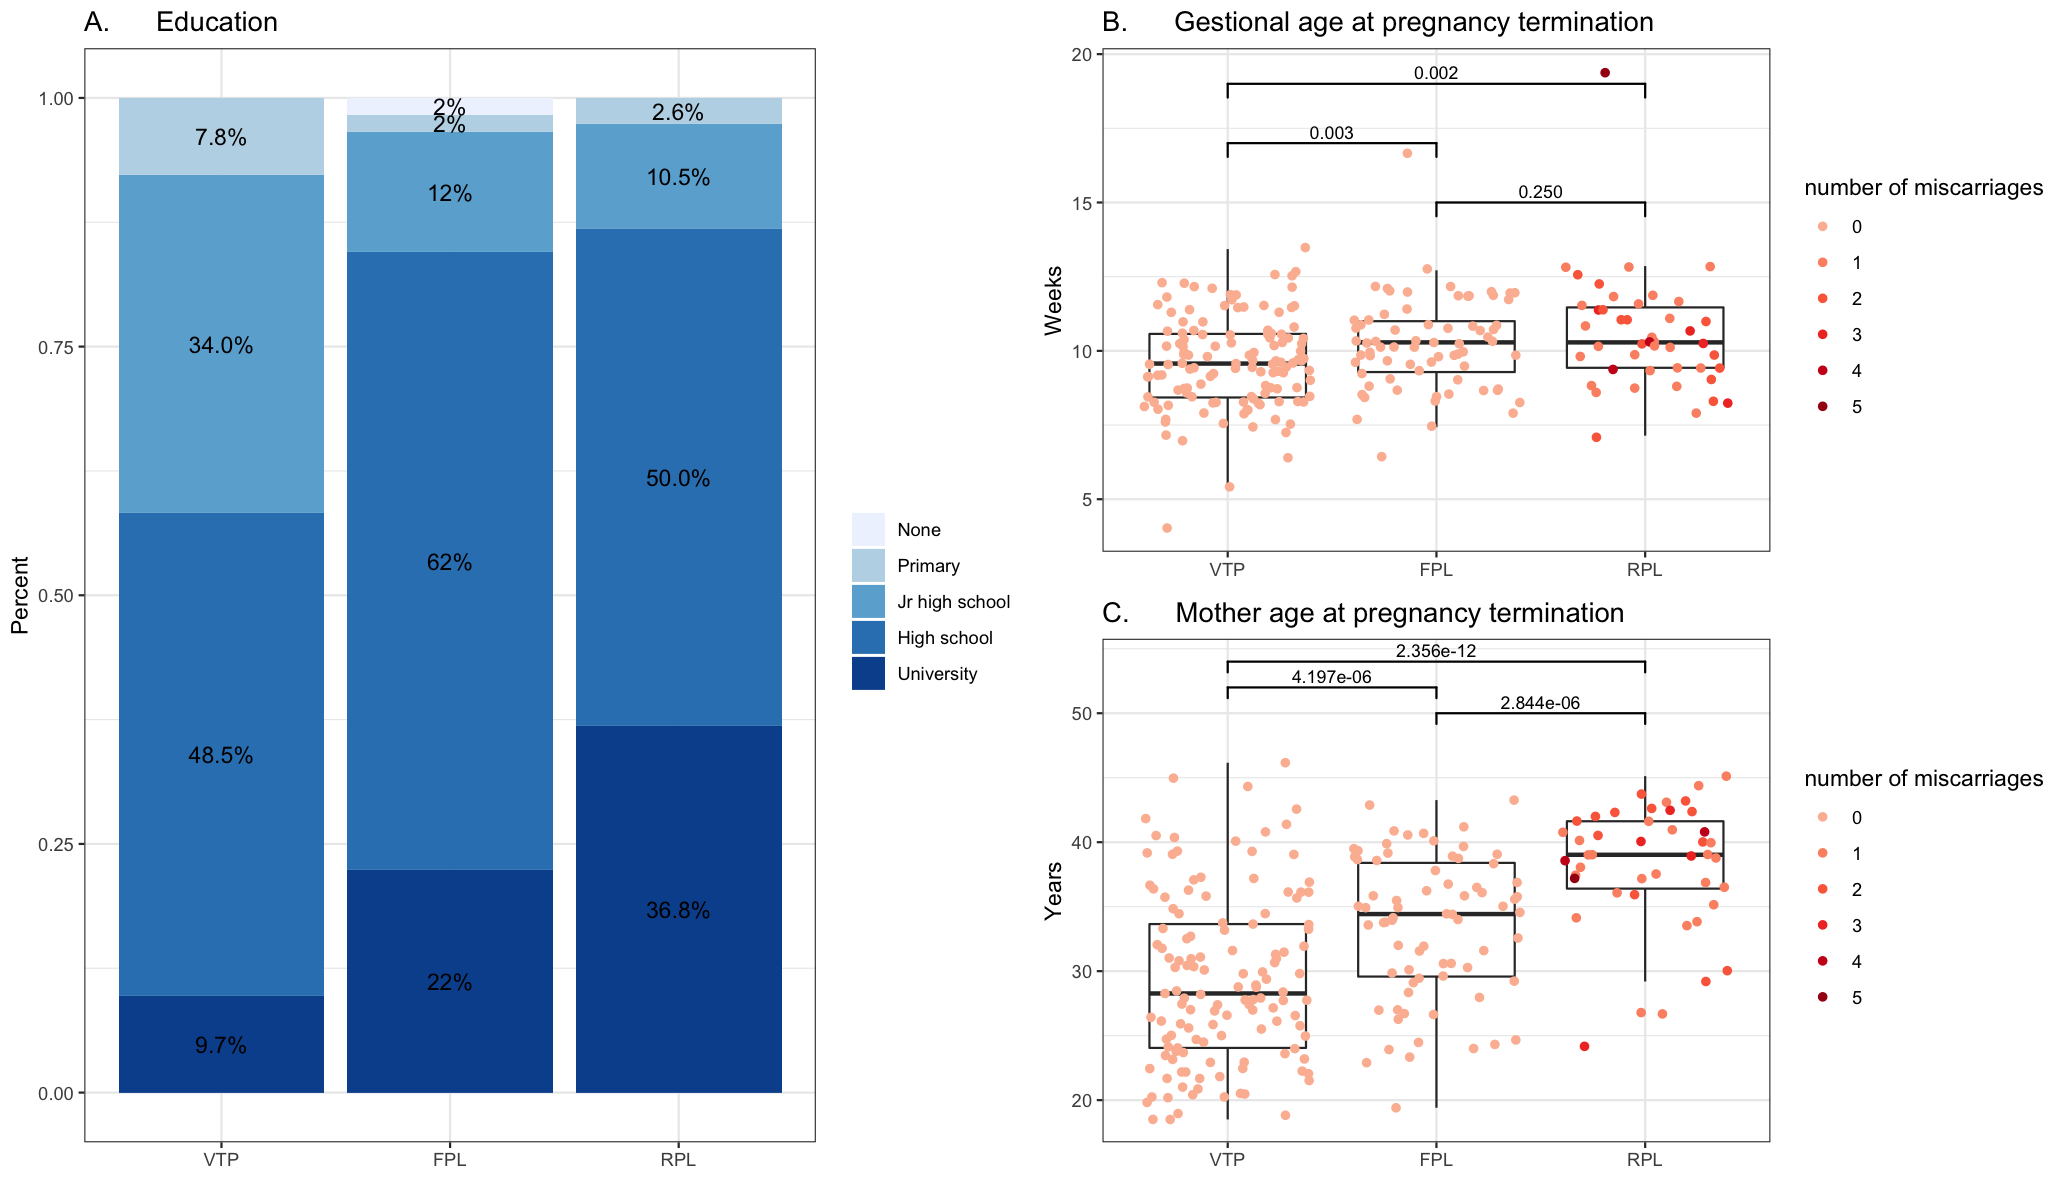
\includegraphics[width=1.10\textwidth]{fig/panel_edu_gestAge_mothAge.png}
\decoRule
\caption{\textbf{Fig A: Education.} RPL samples tend to have higher educational level compared to VTP, probably due high age at first pregnancy of educated woman. \textbf{Fig B:Gestational age at pregnancy termination.} The age of the embryo in PLs range from 4 to 19.4 weeks and there are no significant differences between pairs of classes. \textbf{Fig C: Age of the mother.} Median age of the mother at the event is significantly higher
in RPL compared to FPL.}
\label{fig:panel_edu_gestAge_mothAge}
\end{figure}



Consistently, the median mother age at pregnancy termination is higher in RPL compared to FPL, suggesting that recurrent miscarriages happen more often at advanced age (Figure \ref{fig:panel_edu_gestAge_mothAge}.C, Mann-Whitney p-value\textsubscript{ FPL-RPL}= 2.84e10\textsuperscript{6}). Moving medical parameters, we see no significant differences between RPL, FPL and VTP in terms of Body Mass Index (Figure \ref{fig:panel_BMI_MenAge}.B, Mann-Whitney p-value\textsubscript{ FPL-RPL}= 0.675, p-value\textsubscript{ VTP-FPL}= 0.485, p-value\textsubscript{ VTP-RPL}= 0.620 ), while we observe a wider range of the age at menarche in RPL (8-17 years old) compared to FPL and VTP (Figure \ref{fig:panel_BMI_MenAge}.A, F-test p-value\textsubscript{ VTP-RPL}= 0.0016, p-value\textsubscript{ FPL-RPL}= 0.0288 ).  \newline



\begin{figure}[H]
\centering
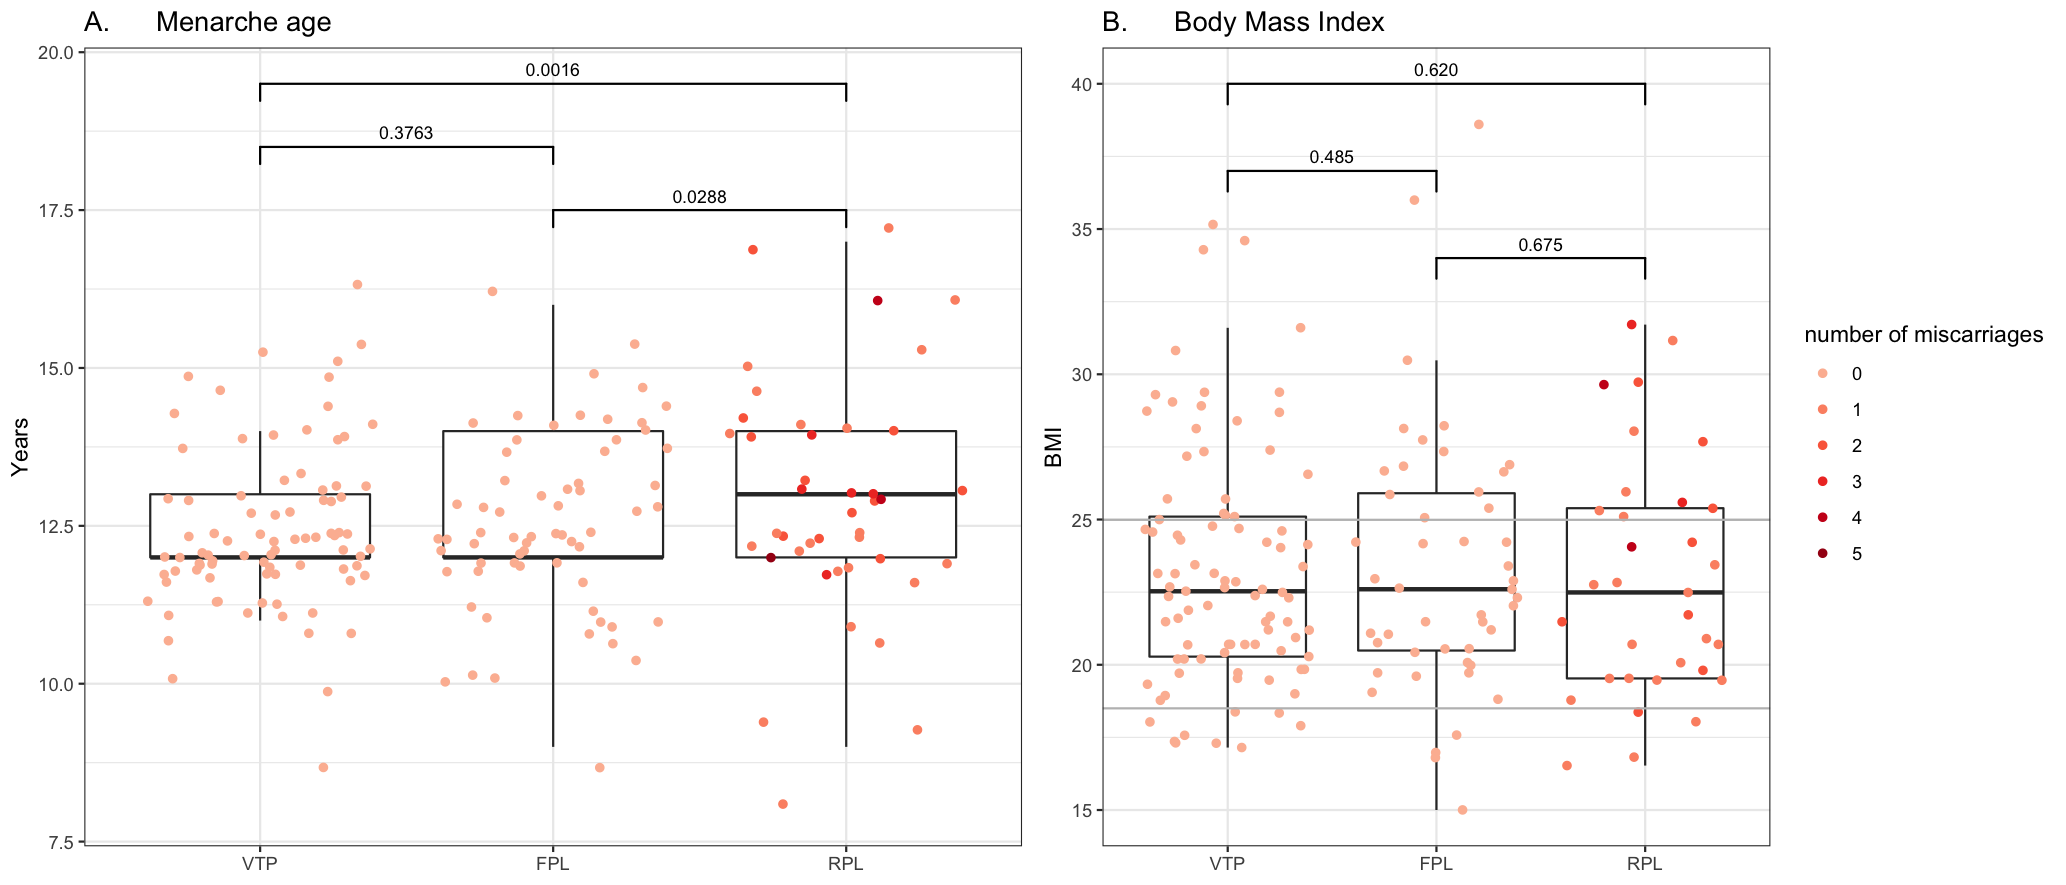
\includegraphics[width=1.15\textwidth]{fig/panel_BMI_MenAge.png}
\decoRule
\caption{\textbf{Fig A:} Age of the menarche is significantly wider in RPL compared to FPL and VTP. \textbf{Fig B:} BMI does not influence pregnancy loss compared to VTP.}
\label{fig:panel_BMI_MenAge}
\end{figure}


%Overall we demonstrate that our data set complies to the standard.. DIsCUSSION 

%%%%%%%%%%%%%%%%%%%%%%%%%%%%%%%%%%%%%%%%%%%%%%%%%%%%%%%%%%%%%%%%%%%%%%%%%%%%%%%%%%%%%%%%%%%%%
%  Section 
%%%%%%%%%%%%%%%%%%%%%%%%%%%%%%%%%%%%%%%%%%%%%%%%%%%%%%%%%%%%%%%%%%%%%%%%%%%%%%%%%%%%%%%%%%%%%

\section{Identification of euploid samples for genetic analyses}
In half of the pregnancies in the first trimester, the causes of PL are large chromosomal aneuploidies, such as trisomies or deletions of large chromosomal chunks \cite{goddijn2000genetic,zhang2009genetic}. With this project, we want to focus on cases in which the embryo is euploid when analyzed with current diagnostic techniques i.e. comparative genomic hybridization (arrayCGH). Hence, samples were screened for chromosomal aneuploidies prior to whole-genome sequencing. This task was performed before my thesis work started, nevertheless, I am describing it here because of its importance. \\

In 44 samples when screened for maternal contamination 11.4\% drops off the analysis, due to technical challenges during sample collection. The first round of detection of aneuploidies on chromosomes 13, 15, 16, 18, 21, 22, X, and Y through Short Tandem Repeats analysis discarded 47.7\% of samples. These types of repeats (tetra- or penta-nucleotide) are often expected to be found in heterozygosis, therefore triploidy is assumed when three alleles are found at several markers along a chromosome (complete) or part of it (partial). Similarly, uniparental disomy for a targeted region or chromosome is assumed when only one parental allele is amplified. Subsequent analysis through array-CGH and \gls{copy number variation} detection form low-coverage sequencing discarded another 11.4\% of samples (Figure \ref{fig:pipelineOutcome}).

The most common aneuploidy in our data set is the trisomy of chromosome 22 (15.9\%), followed by trisomy of chromosome 16 (9\%)(Figure \ref{fig:preseqOutcome}).\newline

Overall 29.5\% of samples were euploid (Figure \ref{fig:preseqOutcome}) and could proceed to whole-genome sequence analysis. By the time I started my thesis I had access to six samples for which sequence data was ready and available to be sequenced. 

\begin{figure}[H]
\centering
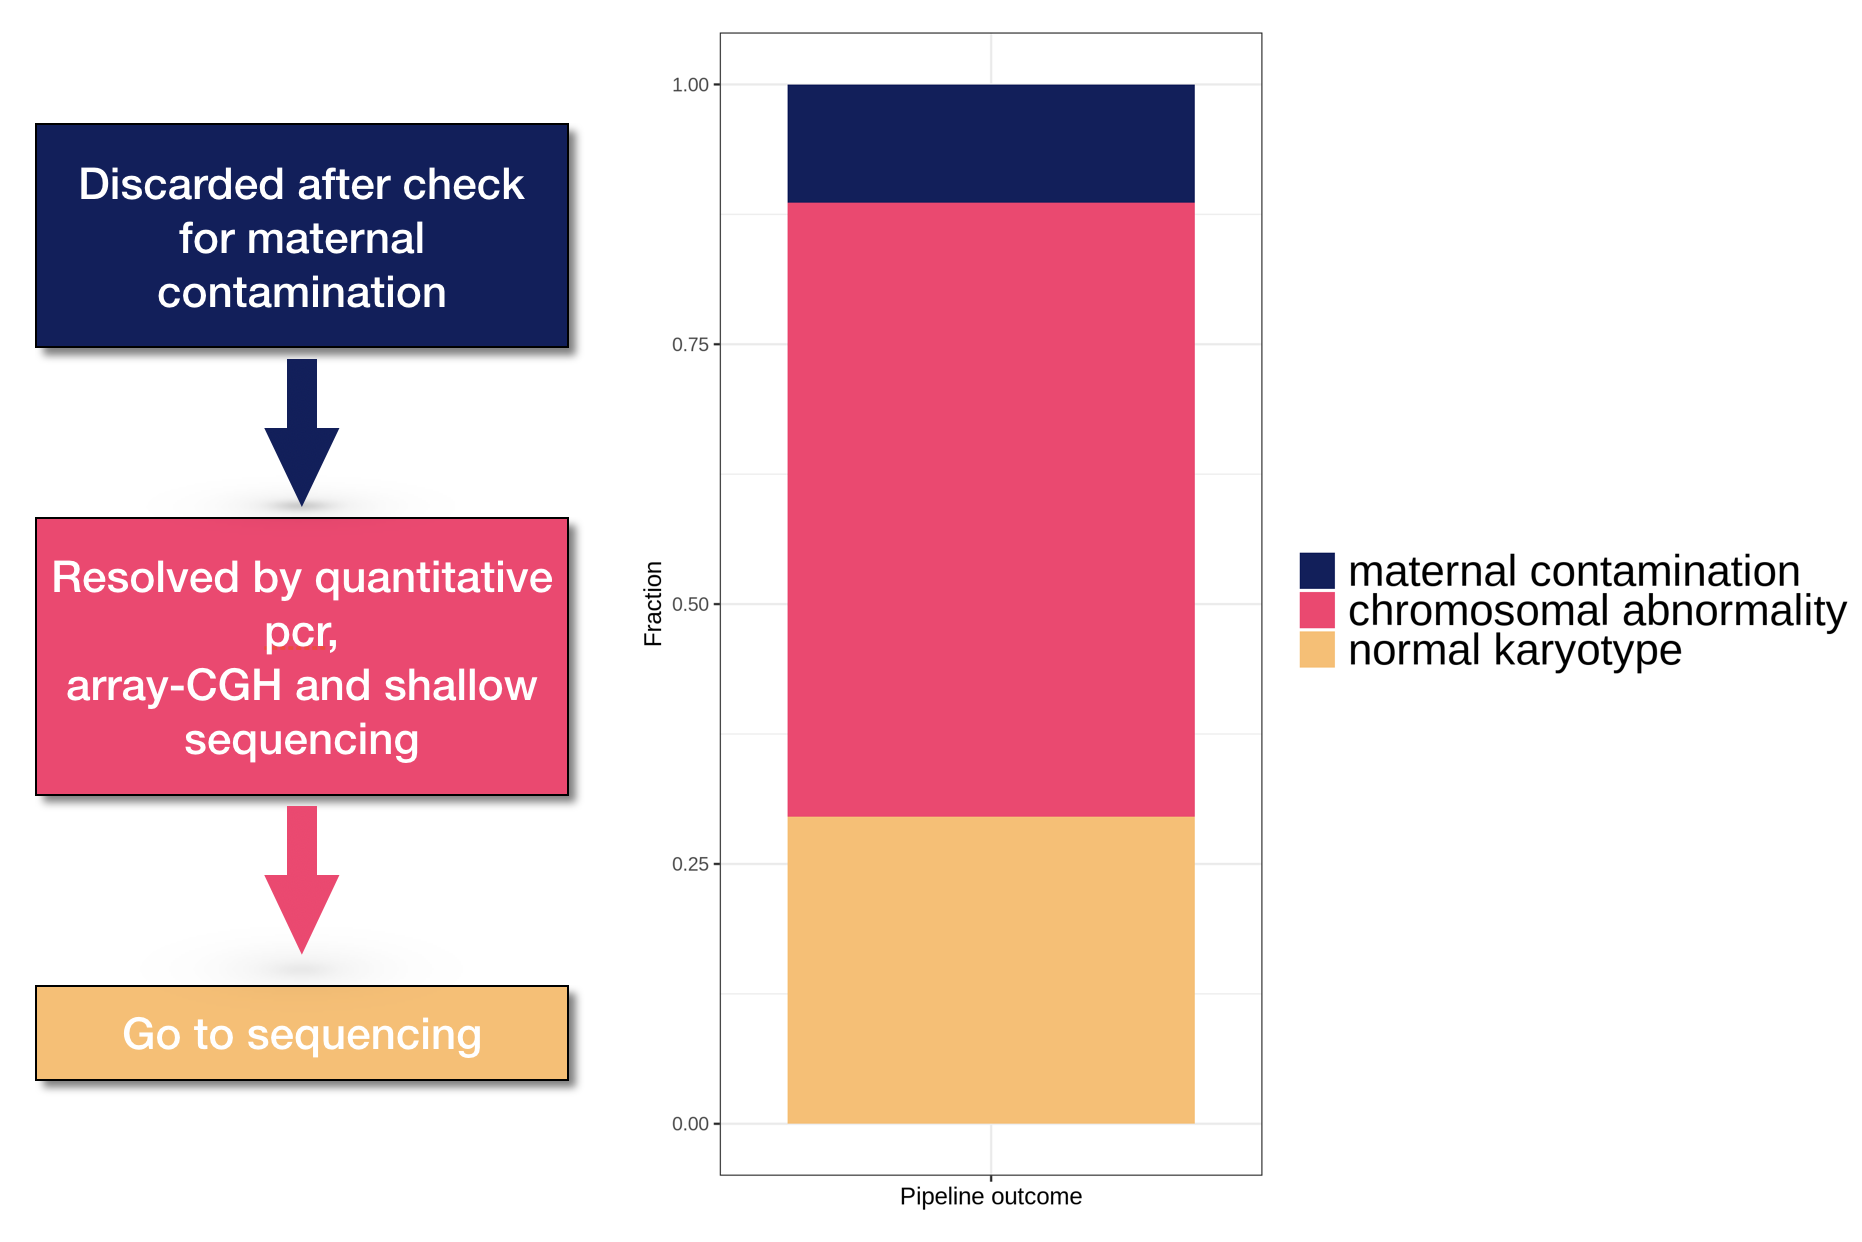
\includegraphics[width=0.7\textwidth]{fig/sampletocollectG.png}
\decoRule
\caption{\textbf{Pre-sequencing screening outcome.} Approximately 10\% of samples are discarded due to maternal contamination, and 60\% for aneuploidies. Finally ~30\% of cases are euploid and proceed to sequencing.}
\label{fig:pipelineOutcome}
\end{figure}

\begin{figure}[H]
\centering
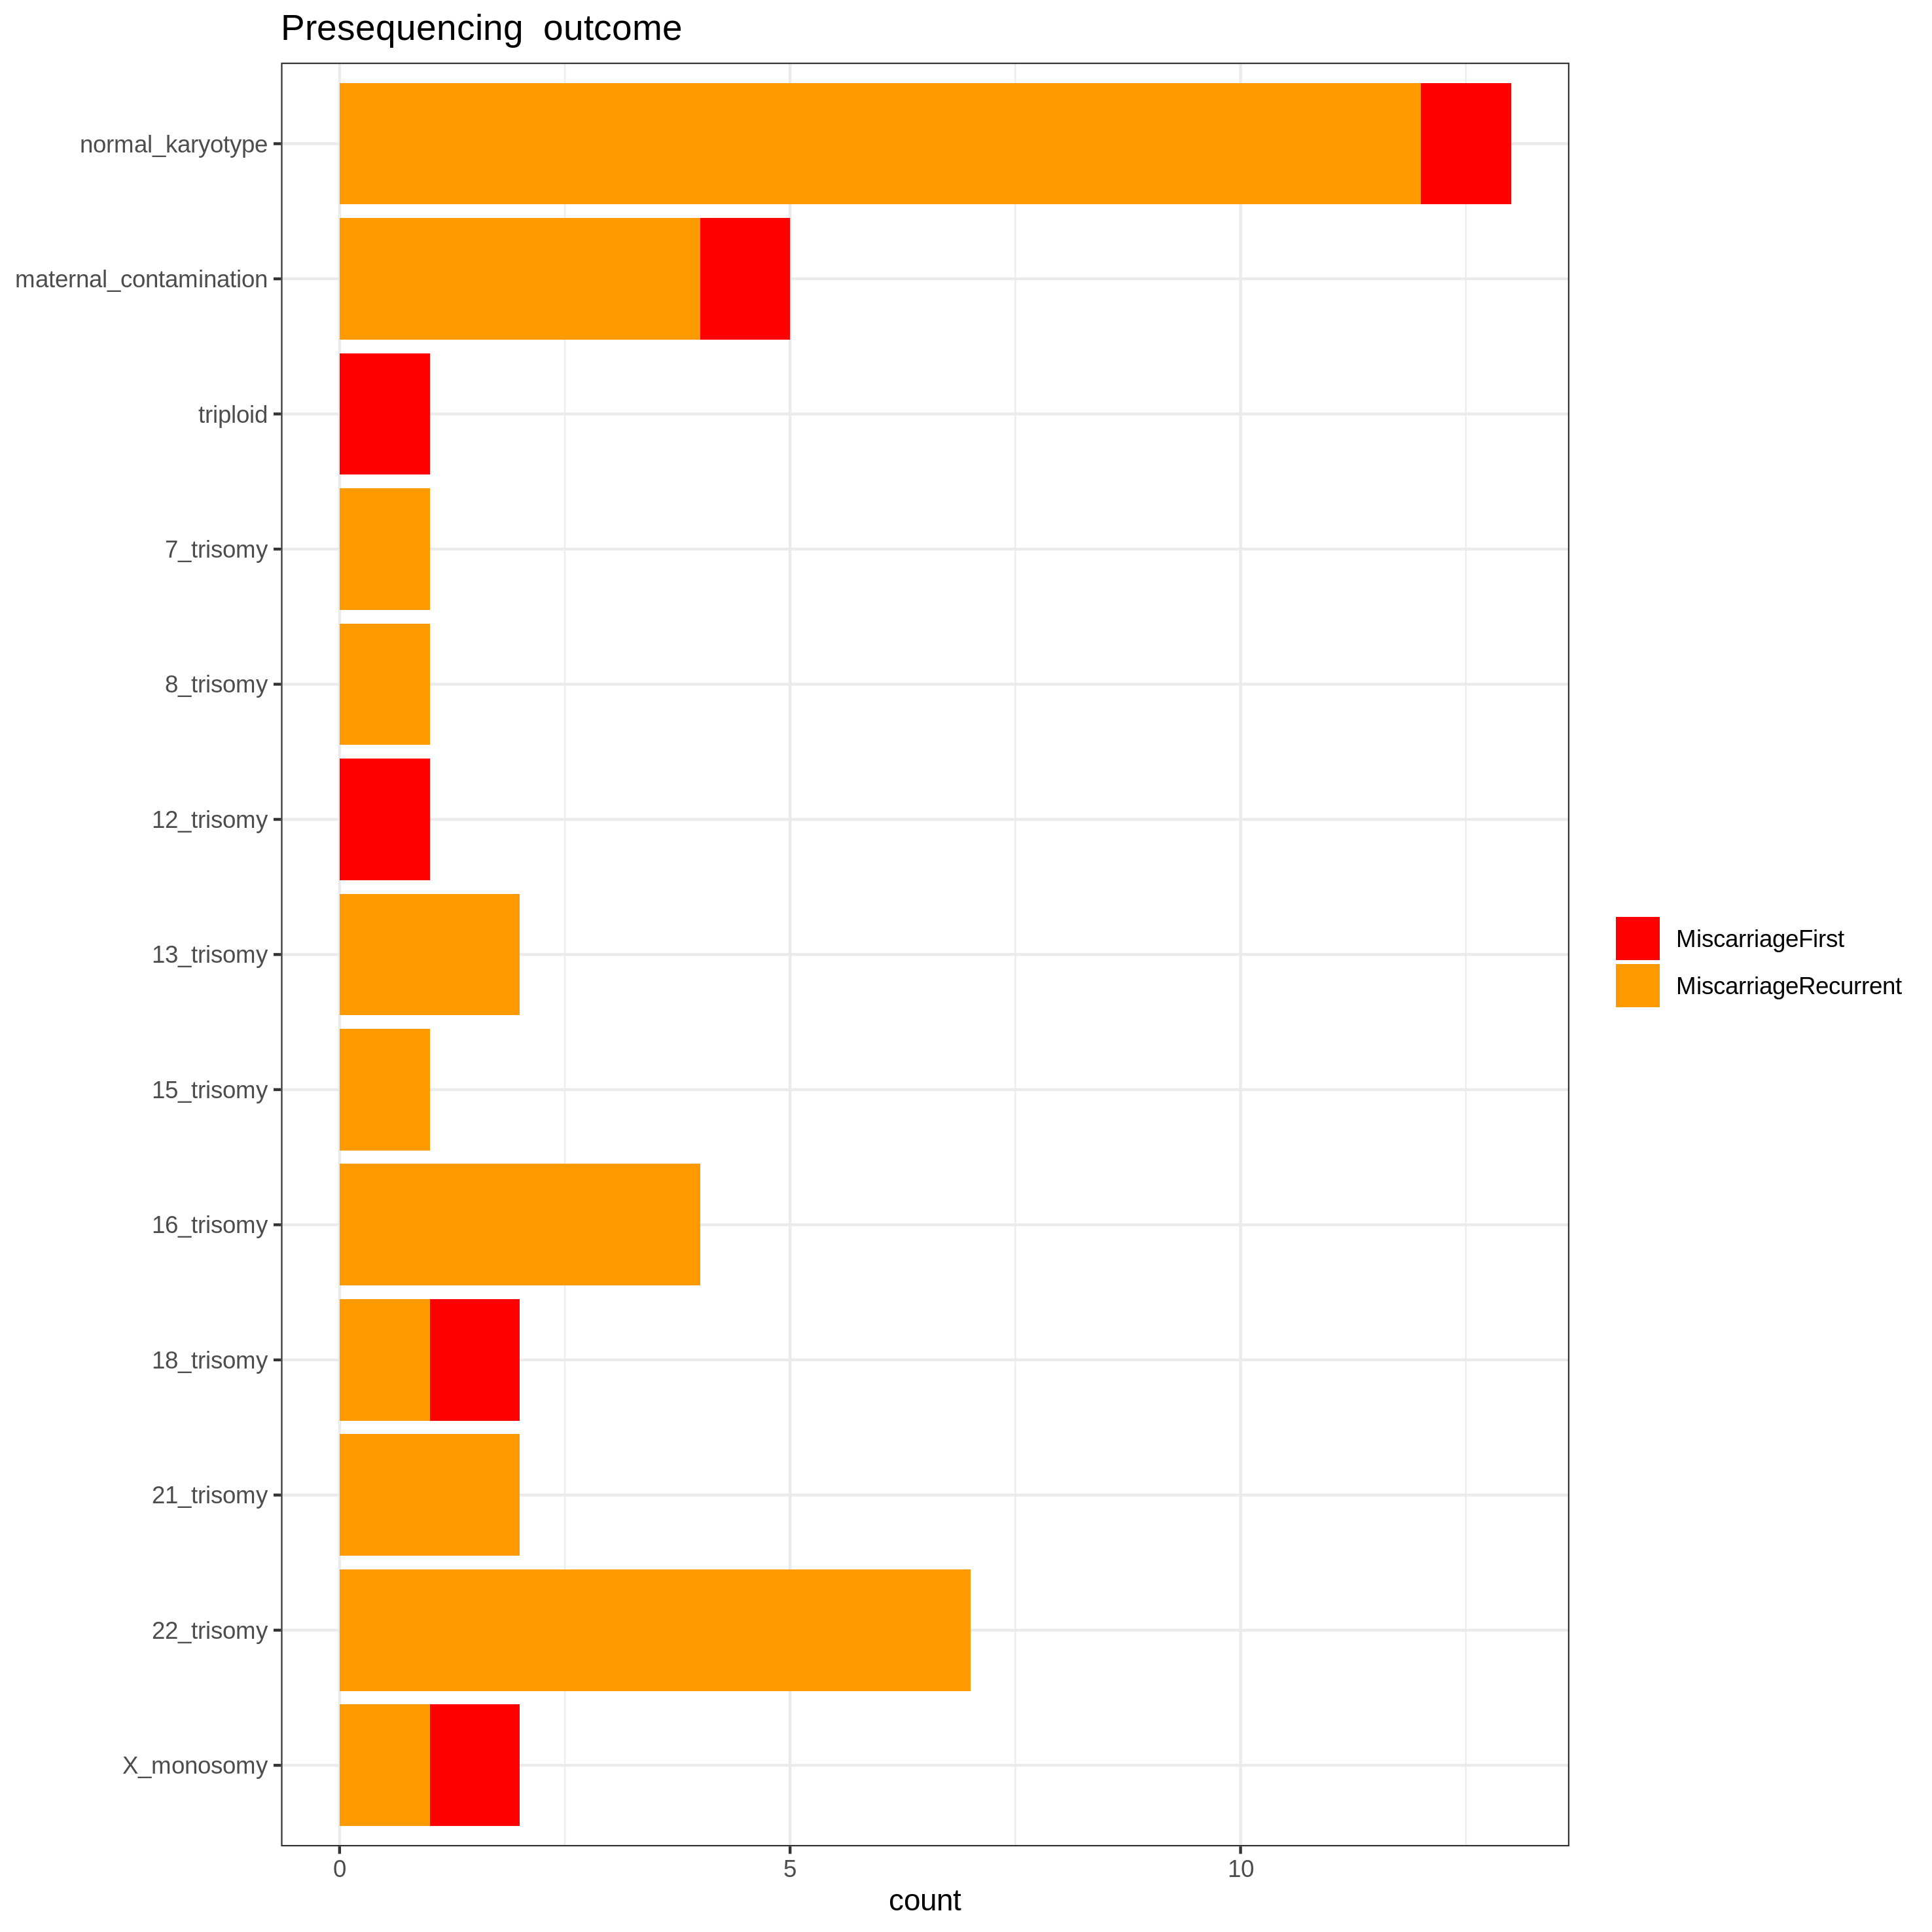
\includegraphics[width=0.8\textwidth]{fig/preseqOutcome.png}
\decoRule
\caption{\textbf{Chromosomal aneuploidies detected in the embryos.} The most common aneuploidies are trisomy on chromosome 22 followed by trisomy on chromosome 16.}
\label{fig:preseqOutcome}
\end{figure}


%%%%%%%%%%%%%%%%%%%%%%%%%%%%%%%%%%%%%%%%%%%%%%%%%%%%%%%%%%%%%%%%%%%%%%%%%%%%%%%%%%%%%%%%%%
%  Section 
%%%%%%%%%%%%%%%%%%%%%%%%%%%%%%%%%%%%%%%%%%%%%%%%%%%%%%%%%%%%%%%%%%%%%%%%%%%%%%%%%%%%%%%%%%

\section{Analysis of whole-genome sequence of embryos from pregnancy loss}
\subsection{Pipeline for the identification of genetic variants}
The sequencing pipeline produces sequence data in the \gls{fastq} format that constitutes the raw sequence data and can be used to perform the analysis from scratch and customized pipelines on \gls{high performance computing} machines. Figure \ref{fig:align-ref-vc} provides an overview of the pipeline used in this study.\newline

\vspace{1cm}

\begin{figure}[H]
\centering
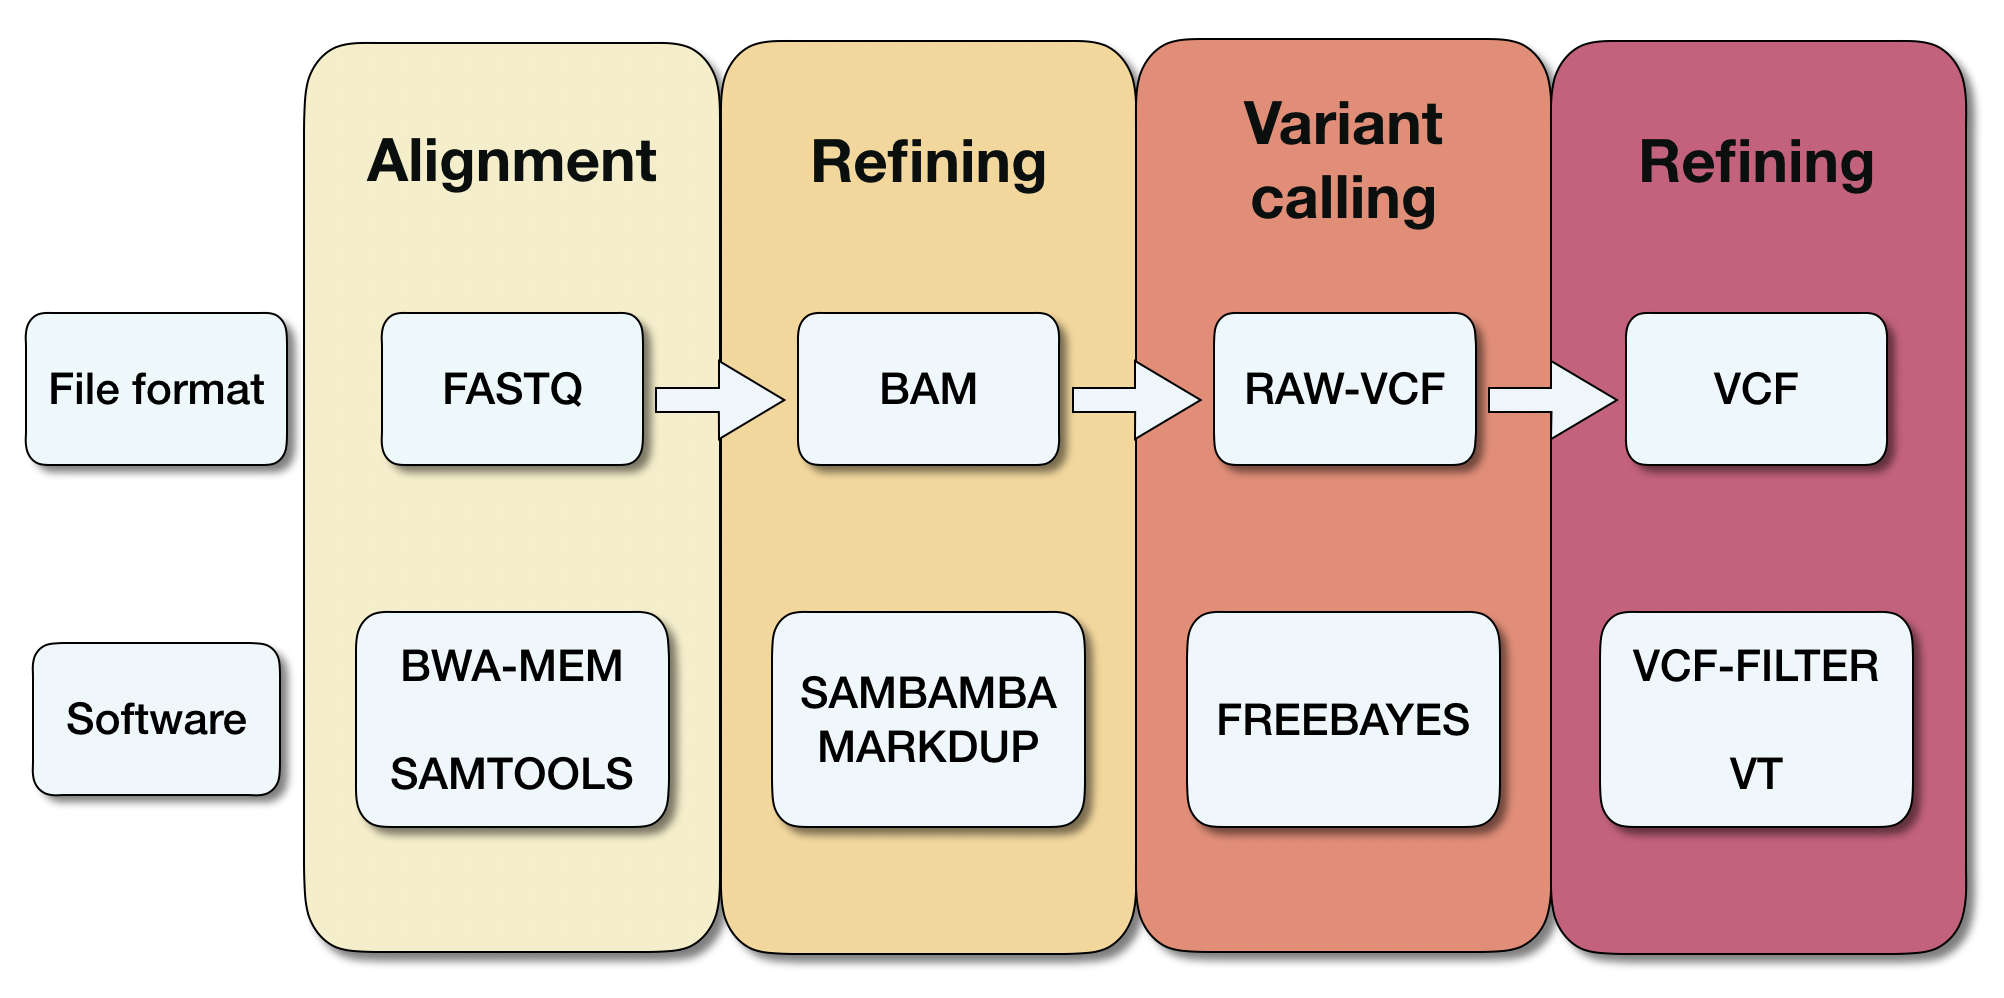
\includegraphics[width=0.7\textwidth]{fig/align-ref-vc.png}
\decoRule
\caption{\textbf{Pipeline for identification of genetic variants.} Sequencing reads are stored in fastq files. The first step is the \textit{alignment} of the reads against the reference genome that produces a bam file. Aligned reads are \textit{refined} and used for \textit{variant calling} that produces vcf files.}
\label{fig:align-ref-vc}
\end{figure}

\vspace{0.5cm}

I performed the \textbf{alignment} of the raw sequence data in form of \gls{reads} against the human reference Genome (GRChg38.p12, \cite{rosenbloom2015ucsc}) using \textsc{bwa-mem} \cite{li2013aligning} and \textsc{samtools} \cite{li2009sequence}. The alignment produces files in the \gls{bam} format that provide information on the quality of the alignemnt and enable some quality controls. In our data set the majority of the reads were correctly aligned to the reference genome.  \newline
Before proceeding to the next step I used \textsc{sambamba} \cite{tarasov2015sambamba} to \textbf{refine} the data and remove PCR duplicates, i.e. reads and they came from the same DNA fragment that bias variant detection through increased homozygosity.\newline

I used the refined bam file to perform \textbf{variant calling} using \textsc{freebayes} \cite{garrison2012haplotype} that produces data in the \gls{vcf} format. The variant calling is the process of identification of variants from sequence data, where variants are chunks of sequence that differ from the reference genome. Genetic variants are classified as single nucleotide variants (SNVs), small insertions and deletions (indels), and structural variants (SVs, large genomic rearrangements). In addition, to call variants, the software specifies whether samples are homozygous or heterozygous (genotype) at the variable sites and the \gls{genotype likelihood}, i.e. the probability that the observed genotype is correct. \newline

The final step is a second round of \textbf{refining} that includes three steps. 
\begin{itemize}
    \item I used \textsc{vcffilter} \cite{vcflib} to filter variants for \gls{quality score}(QUAL)>20. The QUAL is an estimate of how likely it is to observe a call by chance, and a value of 20 corresponds to 1\% probability of having an incorrect genotype.\\
    \item I used \textsc{vt} \cite{tan2015unified} to do the normalization that consist of two parts: parsimony and left alignment. Parsimony is the representation of a variant in as few nucleotides as possible without reducing the length of any allele to 0. Left alignment is the shift of the start position of a variant to the left till it is no longer possible to do so (Figure \ref{fig:vtNorm} \cite{tan2015unified}).\\



    \item I used \textsc{vt} to deconstruct multiallelic variants in a VCF to allow for allelic comparisons between call sets (Figure \ref{fig:vtDecomp}) \cite{tan2015unified}.\\
\end{itemize}

Overall, the variant calling identified on average 4.7M variant site \textit{per} sample. This number corresponds to the expectation in individuals of European ancestry \cite{1000genome2015global}. The most represented class is single nucleotide variant (83.2\%) followed by insertions (6.85\% ) and deletions (6.84\%)(Figure \ref{fig:variantClass}, \ref{fig:percentVariantClass})

\begin{figure}[H]
\centering
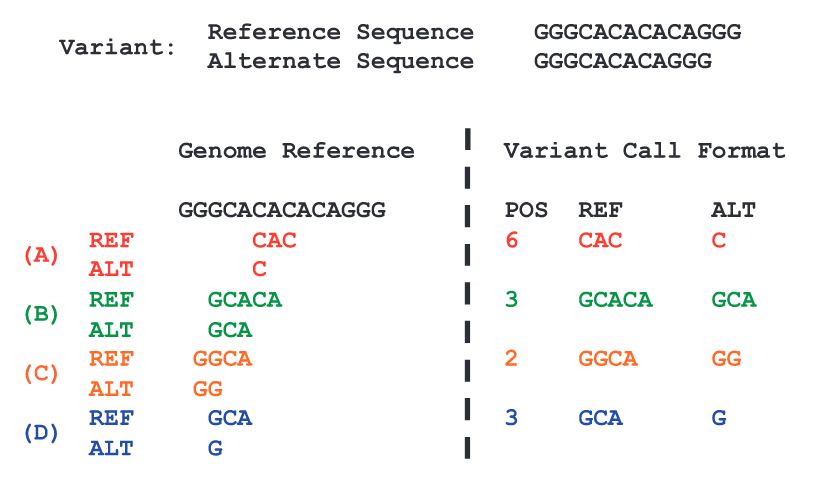
\includegraphics[width=0.55\textwidth]{fig/vtNormalizeTan.png}
\decoRule
\caption{\textbf{Normalization.} Example  of  VCF  entries  representing  the  same  variant. Left  panel aligns each allele to the reference genome, and the right panel represents the variant in VCF. (A) is not left-aligned (B) is neither left-aligned nor parsimonious, (C) is not parsimonious and (D) is normalized. \textit{ Adapted from \cite{tan2015unified}}}
\label{fig:vtNorm}
\end{figure}

\vspace{2cm}

\begin{figure}[H]
\centering
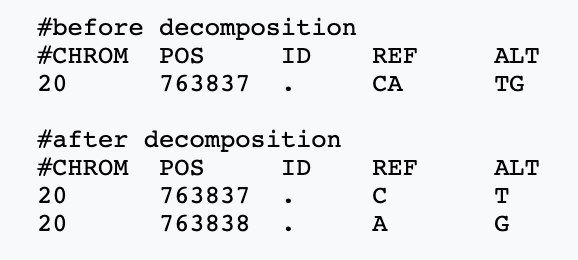
\includegraphics[width=0.55\textwidth]{fig/vtDecompose.png}
\decoRule
\caption{\textbf{Decompositon} Biallelic clumped variant are decomposed for allelic comparisons between call sets} \textit{ Adapted from \cite{tan2015unified}}. 
\label{fig:vtDecomp}
\end{figure}

\begin{figure}[H]
\centering
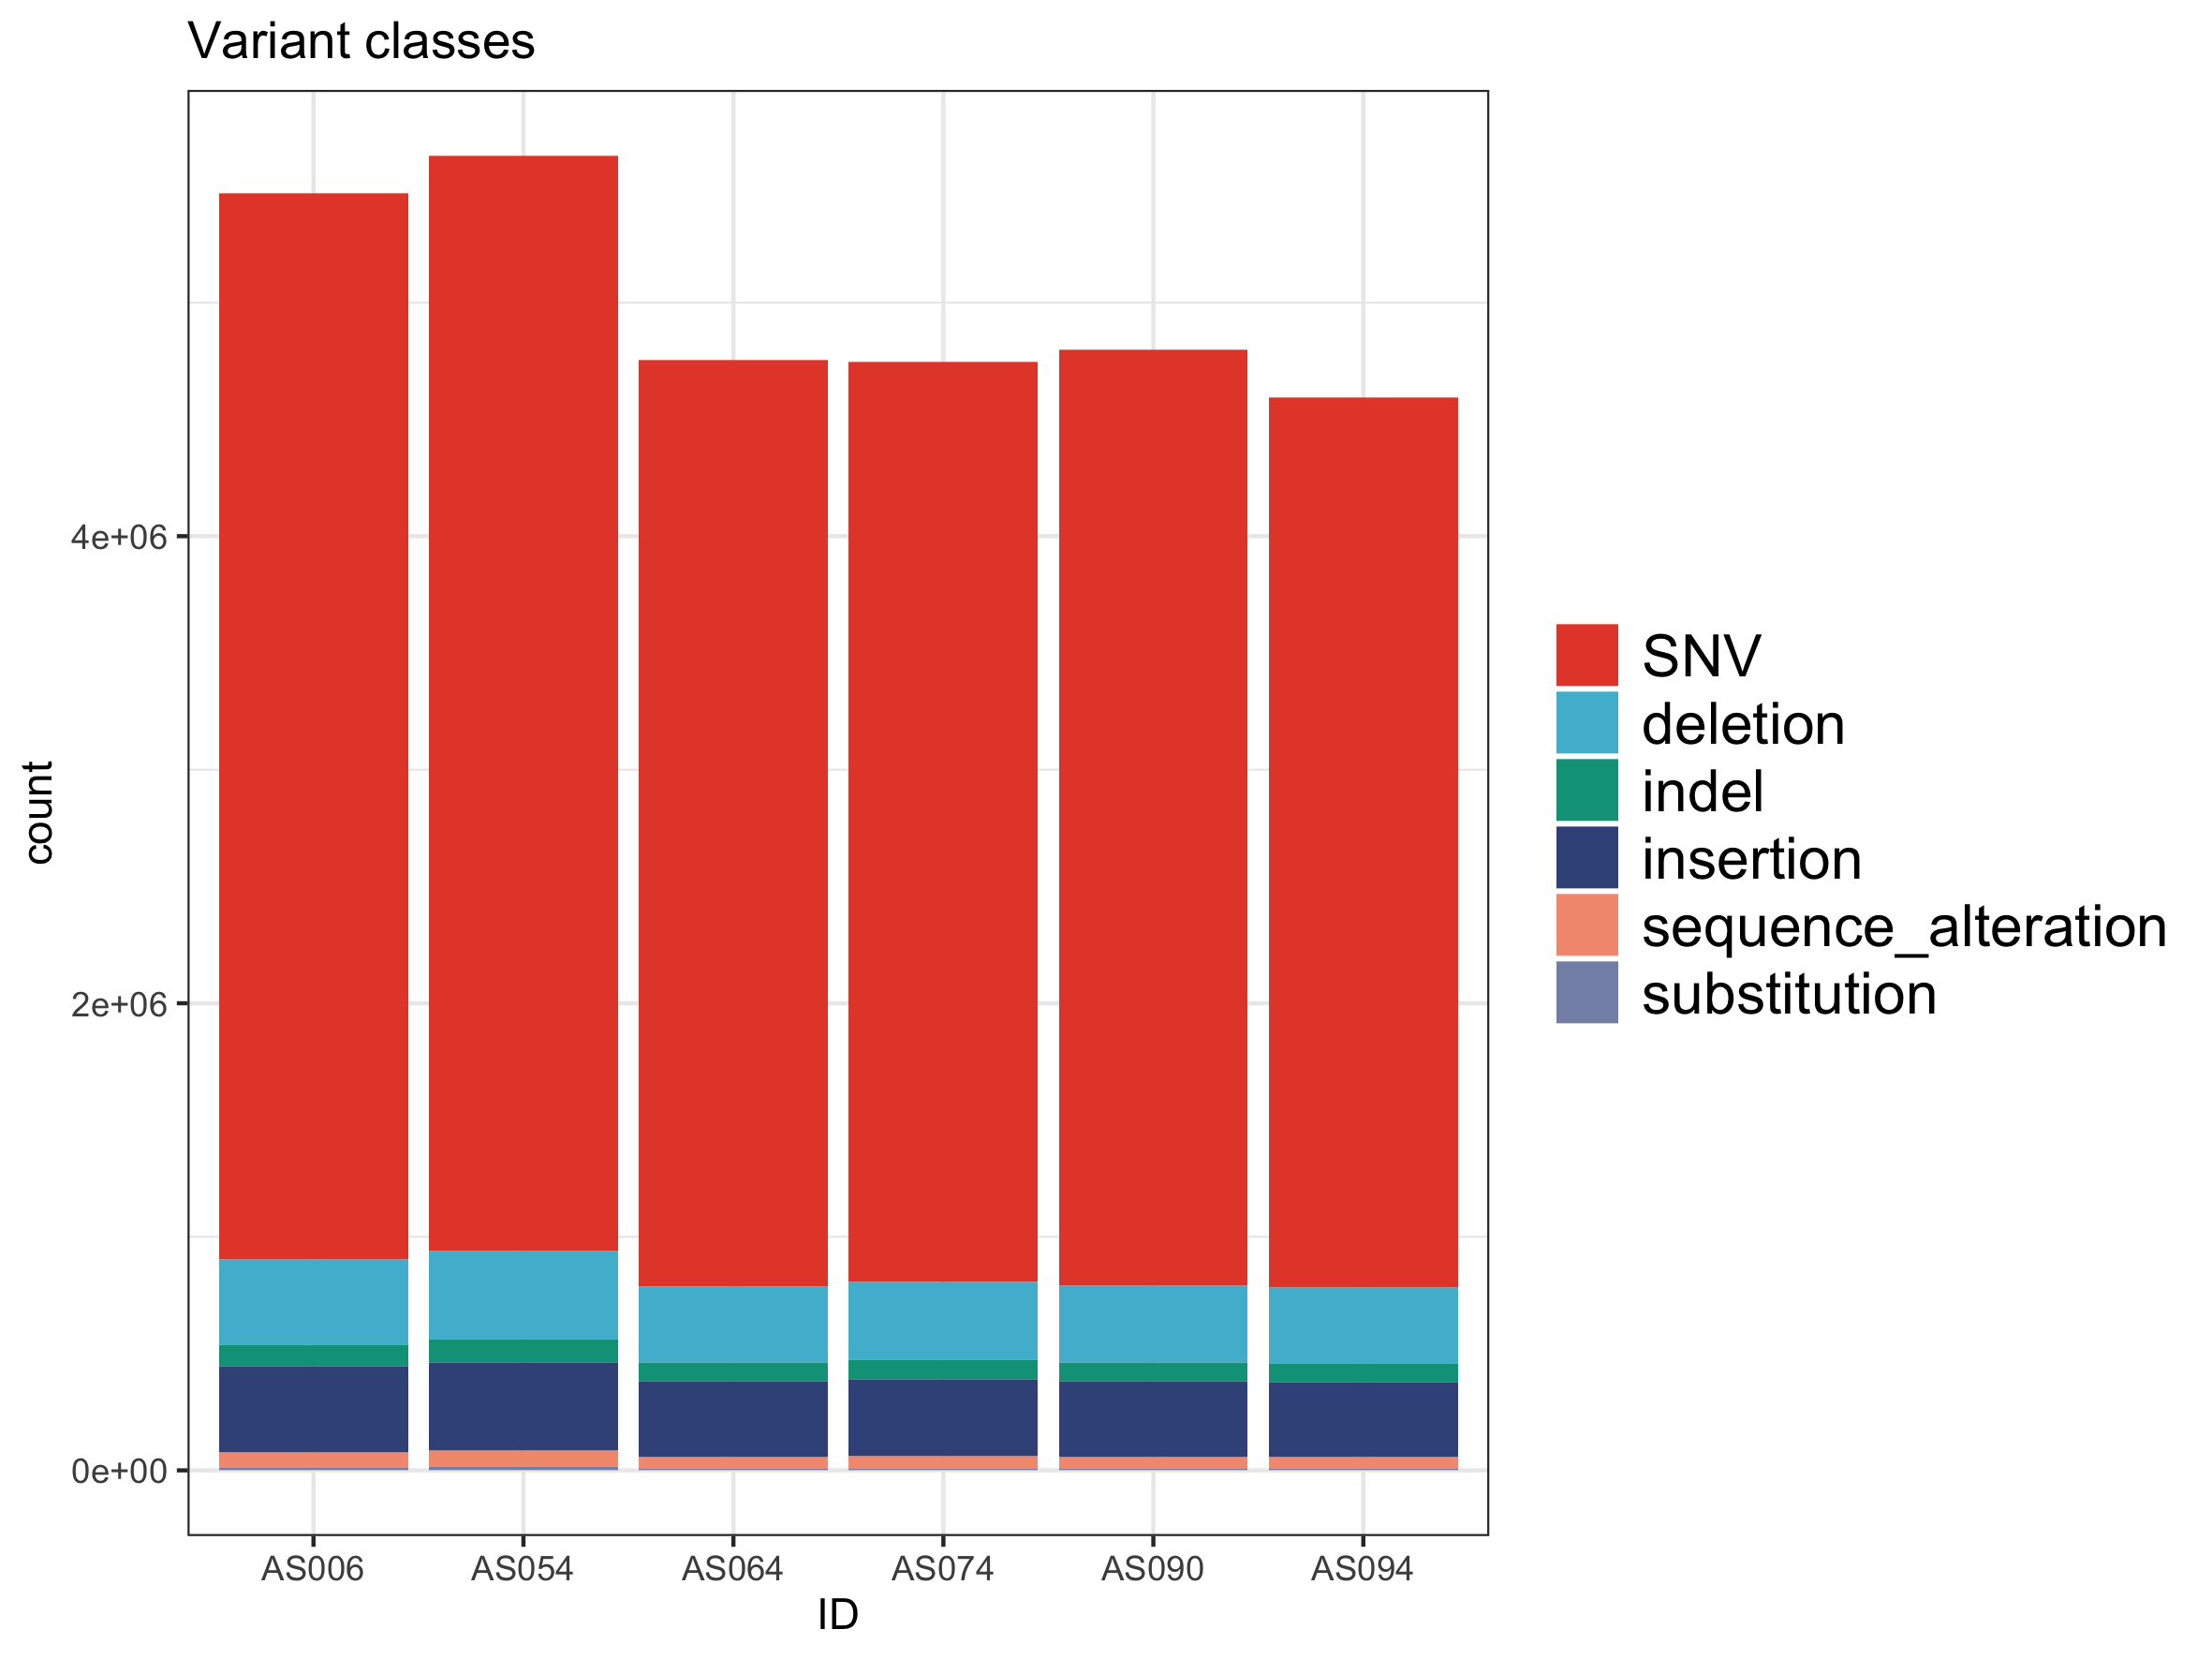
\includegraphics[width=0.55\textwidth]{fig/variantClass.png}
\decoRule
\caption{\textbf{Counts of variants types per sample.} The most represented class is single nucleotide variant (83.2\%) followed by insertions (6.85\% ) and deletions (6.84\% }
\label{fig:variantClass}
\end{figure}

\vspace{1.5cm}

\begin{figure}[H]
\centering
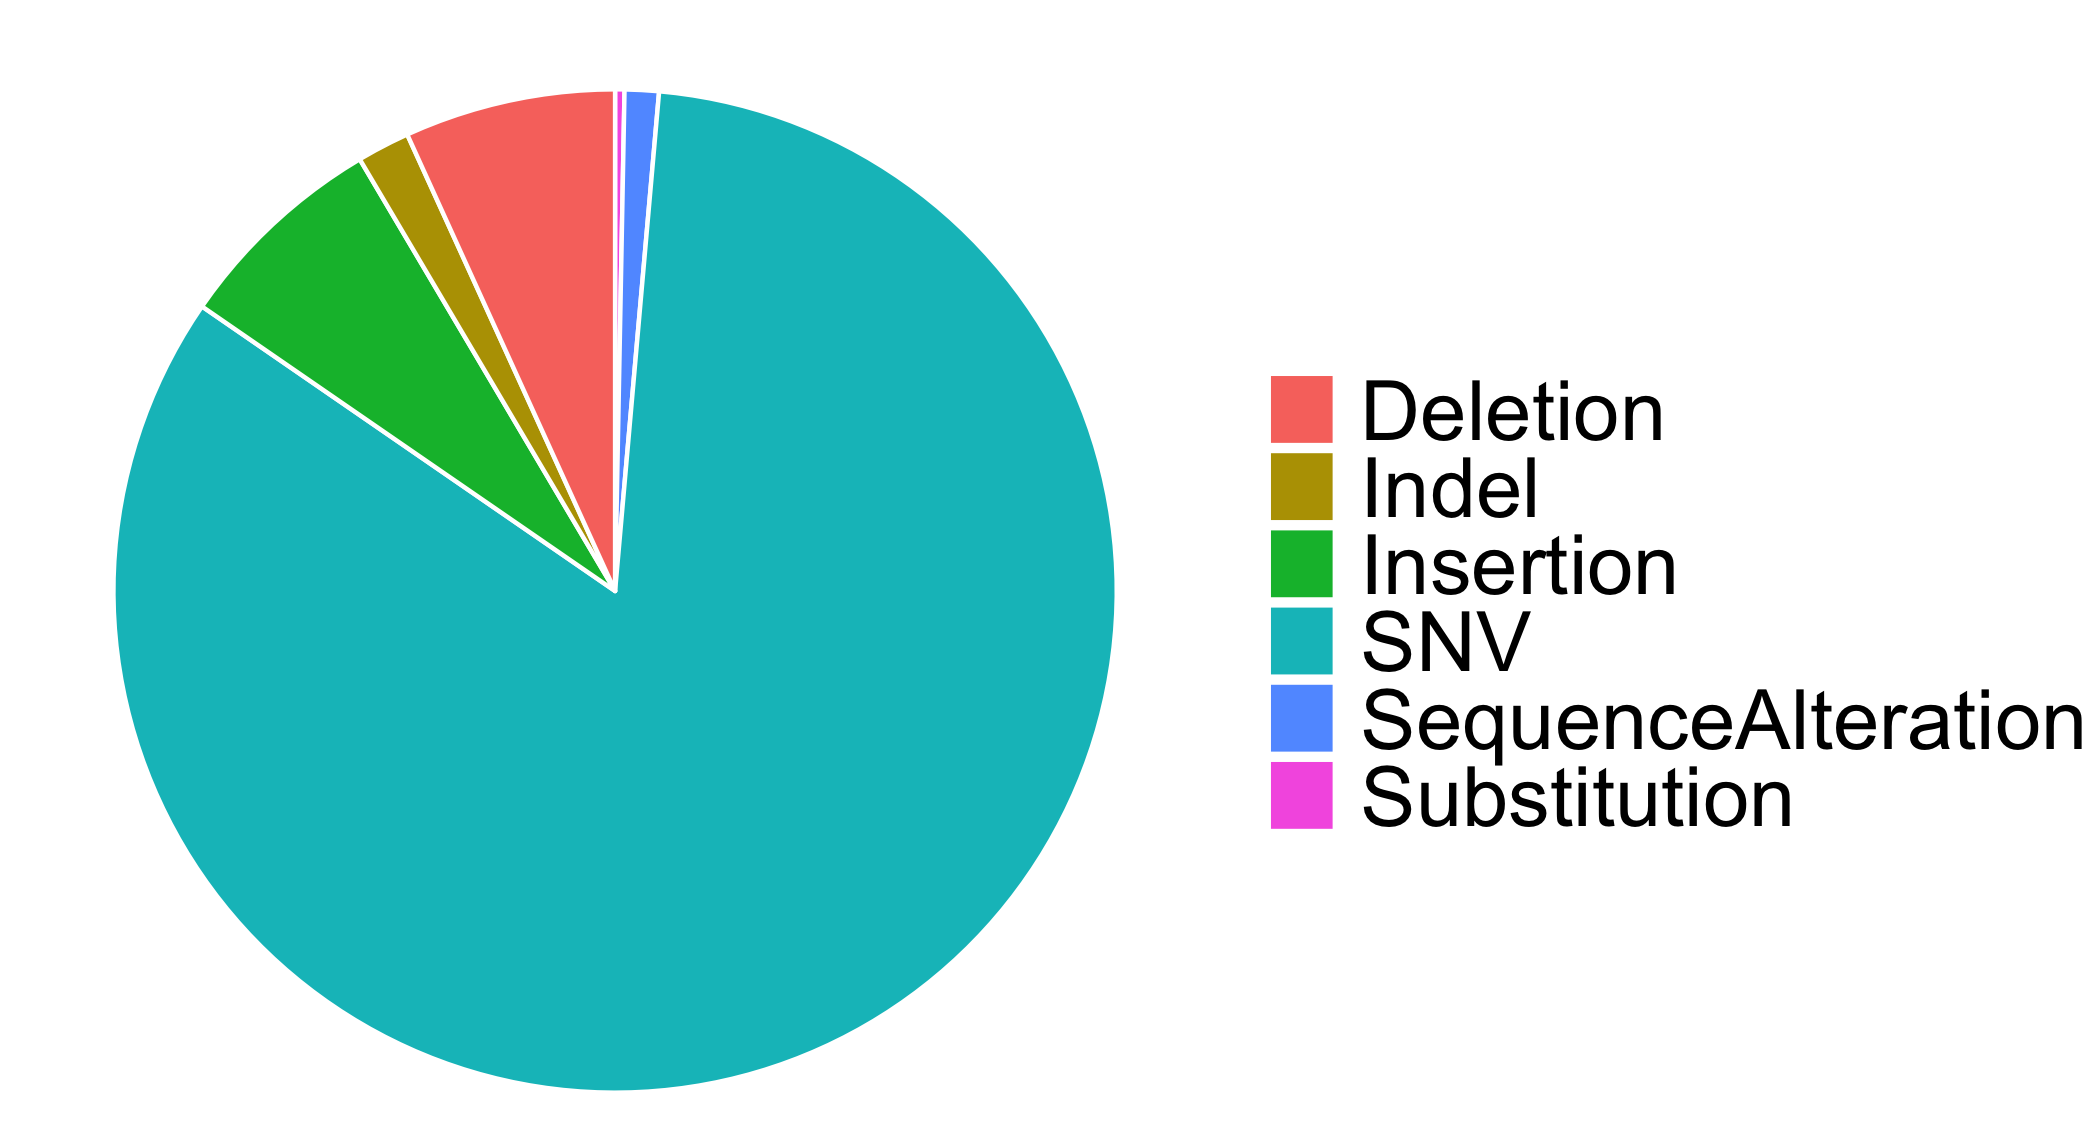
\includegraphics[width=0.55\textwidth]{fig/PieVariantClass.png}
\decoRule
\caption{\textbf{Average prevalence of variant types among samples}. SNV 83.2\%, insertion 6.85\%, deletion 6.84\%, indel 1.7\%, sequence alteration 1.05\%, substitution 0.2\%}
\label{fig:percentVariantClass}
\end{figure}


%%%%%%%%%%%%%%%%%%%%%%%%%%%%%%%%%%%%%%%%%%%%%%%%%%%%%%%%%%%%%%%%%%%%%%%%%%%%%%%%%%%%%%%
%  Subsection 
%%%%%%%%%%%%%%%%%%%%%%%%%%%%%%%%%%%%%%%%%%%%%%%%%%%%%%%%%%%%%%%%%%%%%%%%%%%%%%%%%%%%%%%

\subsection{Functional annotation of genetic variants}

Once the genetic variants are identified, the following challenge is to understand their functional consequences, i.e.the effect that they produce on the gene and if they cause a specific phenotype. I have used \textsc{variant effect predictor} \textsc{vep}, \cite{mclaren2016ensembl} provided by Ensembl \cite{howe2020ensembl} to annotate the genetic variant discovered in the six GREP samples. \textsc{vep} is currently the most updated and comprehensive toolset for the analysis, annotation, and prioritization of genomic variants in the coding and non-coding regions based on an extensive collection of genomic annotations. \textsc{vep} can determine the effect of variants (SNPs, insertions, deletions, CNVs or structural variants) on genes, transcripts, and protein sequence, as well as regulatory regions.\newline

{\small
\begin{sidewaystable}
\caption{Table of Consequences}
\label{tab:csqVEP}
\centering
\begin{adjustbox}{width=1\textwidth}
\begin{tabular}{c c c c}
\toprule
\tabhead{SO term} & \tabhead{SO description} & \tabhead{SO accession} & \tabhead{Impact} \\
\midrule
transcript ablation & A feature ablation whereby the deleted region includes a transcript feature & SO:0001893 & HIGH \\
splice acceptor variant & A splice variant that changes the 2 base region at the 3' end of an intron & SO:0001574 & HIGH \\
splice donor variant & A splice variant that changes the 2 base region at the 5' end of an intron & SO:0001575 & HIGH \\
stop gained & A sequence variant whereby at least one base of a codon is changed, resulting in a premature stop codon, leading to a shortened transcript & SO:0001587 & HIGH \\
frameshift variant & A sequence variant which causes a disruption of the translational reading frame, because the number of nucleotides inserted or deleted is not a multiple of three & SO:0001589 & HIGH \\
stop lost & A sequence variant where at least one base of the terminator codon (stop) is changed, resulting in an elongated transcript & SO:0001578 & HIGH \\
start lost & A codon variant that changes at least one base of the canonical start codon & SO:0002012 & HIGH \\
transcript amplification & A feature amplification of a region containing a transcript & SO:0001889 & HIGH \\
inframe insertion & An inframe non synonymous variant that inserts bases into in the coding sequence & SO:0001821 & MODERATE \\
inframe deletion & An inframe non synonymous variant that deletes bases from the coding sequence & SO:0001822 & MODERATE \\
missense variant & A sequence variant, that changes one or more bases, resulting in a different amino acid sequence but where the length is preserved & SO:0001583 & MODERATE \\
protein altering variant & A sequence variant which is predicted to change the protein encoded in the coding sequence & SO:0001818 & MODERATE \\
splice region variant & A sequence variant in which a change has occurred within the region of the splice site, either within 1-3 bases of the exon or 3-8 bases of the intron & SO:0001630 & LOW \\
incomplete terminal codon variant & A sequence variant where at least one base of the final codon of an incompletely annotated transcript is changed & SO:0001626 & LOW \\
start retained variant & A sequence variant where at least one base in the start codon is changed, but the start remains & SO:0002019 & LOW \\
stop retained variant & A sequence variant where at least one base in the terminator codon is changed, but the terminator remains & SO:0001567 & LOW \\
synonymous variant & A sequence variant where there is no resulting change to the encoded amino acid & SO:0001819 & LOW \\
coding sequence variant & A sequence variant that changes the coding sequence & SO:0001580 & MODIFIER \\
mature miRNA variant & A transcript variant located with the sequence of the mature miRNA & SO:0001620 & MODIFIER \\
5 prime UTR variant & A UTR variant of the 5' UTR & SO:0001623 & MODIFIER \\
3 prime UTR variant & A UTR variant of the 3' UTR & SO:0001624 & MODIFIER \\
non coding transcript exon variant & A sequence variant that changes non-coding exon sequence in a non-coding transcript & SO:0001792 & MODIFIER \\
intron variant & A transcript variant occurring within an intron & SO:0001627 & MODIFIER \\
NMD transcript variant & A variant in a transcript that is the target of NMD & SO:0001621 & MODIFIER \\
non coding transcript variant & A transcript variant of a non coding RNA gene & SO:0001619 & MODIFIER \\
upstream gene variant & A sequence variant located 5' of a gene & SO:0001631 & MODIFIER \\
downstream gene variant & A sequence variant located 3' of a gene & SO:0001632 & MODIFIER \\
TFBS ablation & A feature ablation whereby the deleted region includes a transcription factor binding site & SO:0001895 & MODIFIER \\
TFBS amplification & A feature amplification of a region containing a transcription factor binding site & SO:0001892 & MODIFIER \\
TF binding site variant & A sequence variant located within a transcription factor binding site & SO:0001782 & MODIFIER \\
regulatory region ablation & A feature ablation whereby the deleted region includes a regulatory region & SO:0001894 & MODERATE \\
regulatory region amplification & A feature amplification of a region containing a regulatory region & SO:0001891 & MODIFIER \\
feature elongation & A sequence variant that causes the extension of a genomic feature, with regard to the reference sequence & SO:0001907 & MODIFIER \\
regulatory region variant & A sequence variant located within a regulatory region & SO:0001566 & MODIFIER \\
feature truncation & A sequence variant that causes the reduction of a genomic feature, with regard to the reference sequence & SO:0001906 & MODIFIER \\
intergenic variant & A sequence variant located in the intergenic region, between genes & SO:0001628 & MODIFIER \\
\bottomrule\\
\end{tabular}
\end{adjustbox}
\end{sidewaystable}
}

Table \ref{tab:csqVEP} (adapted from \cite{mclaren2016ensembl}) describes the classification of the consequences in the Ensembl Variation database. The impact of the variant on the gene product is classified into four categories: high, moderate, low, and modifier. Examples of variations with high impact are mutations that cause premature termination of the transcription (stop gained) or that suppress transcription (start lost). The classification includes variants in genic (e.g. missense), regulatory (e.g. located in transcription factor binding site) and intergenic regions. In the analysis of the GREP samples, we refer to these categories. 



Figure \ref{fig:grid_cons} shows the outcome of \textsc{vep} stratified by categories of impact. All sample present very similar patterns as shown in Table \ref{tab:percentageImpact} showing percentage for each category of impact. Among the variants with high impact the most represented is Splice donor variant, followed by Splice acceptor and frameshift variants (Figure \ref{fig:grid_cons}.A). Almost all variants with moderate impact are missense variants (99\%, Figure \ref{fig:grid_cons}.B). Among variants with low impact, there is a prevalence of synonymous (68.5\%) and splice region (31.3\%) variants. Finally, the more common variants among modifiers are intron (50.6\%) and intergenic (34.8\%) variants. 

\vspace{1cm}

\begin{figure}[H]
\centering
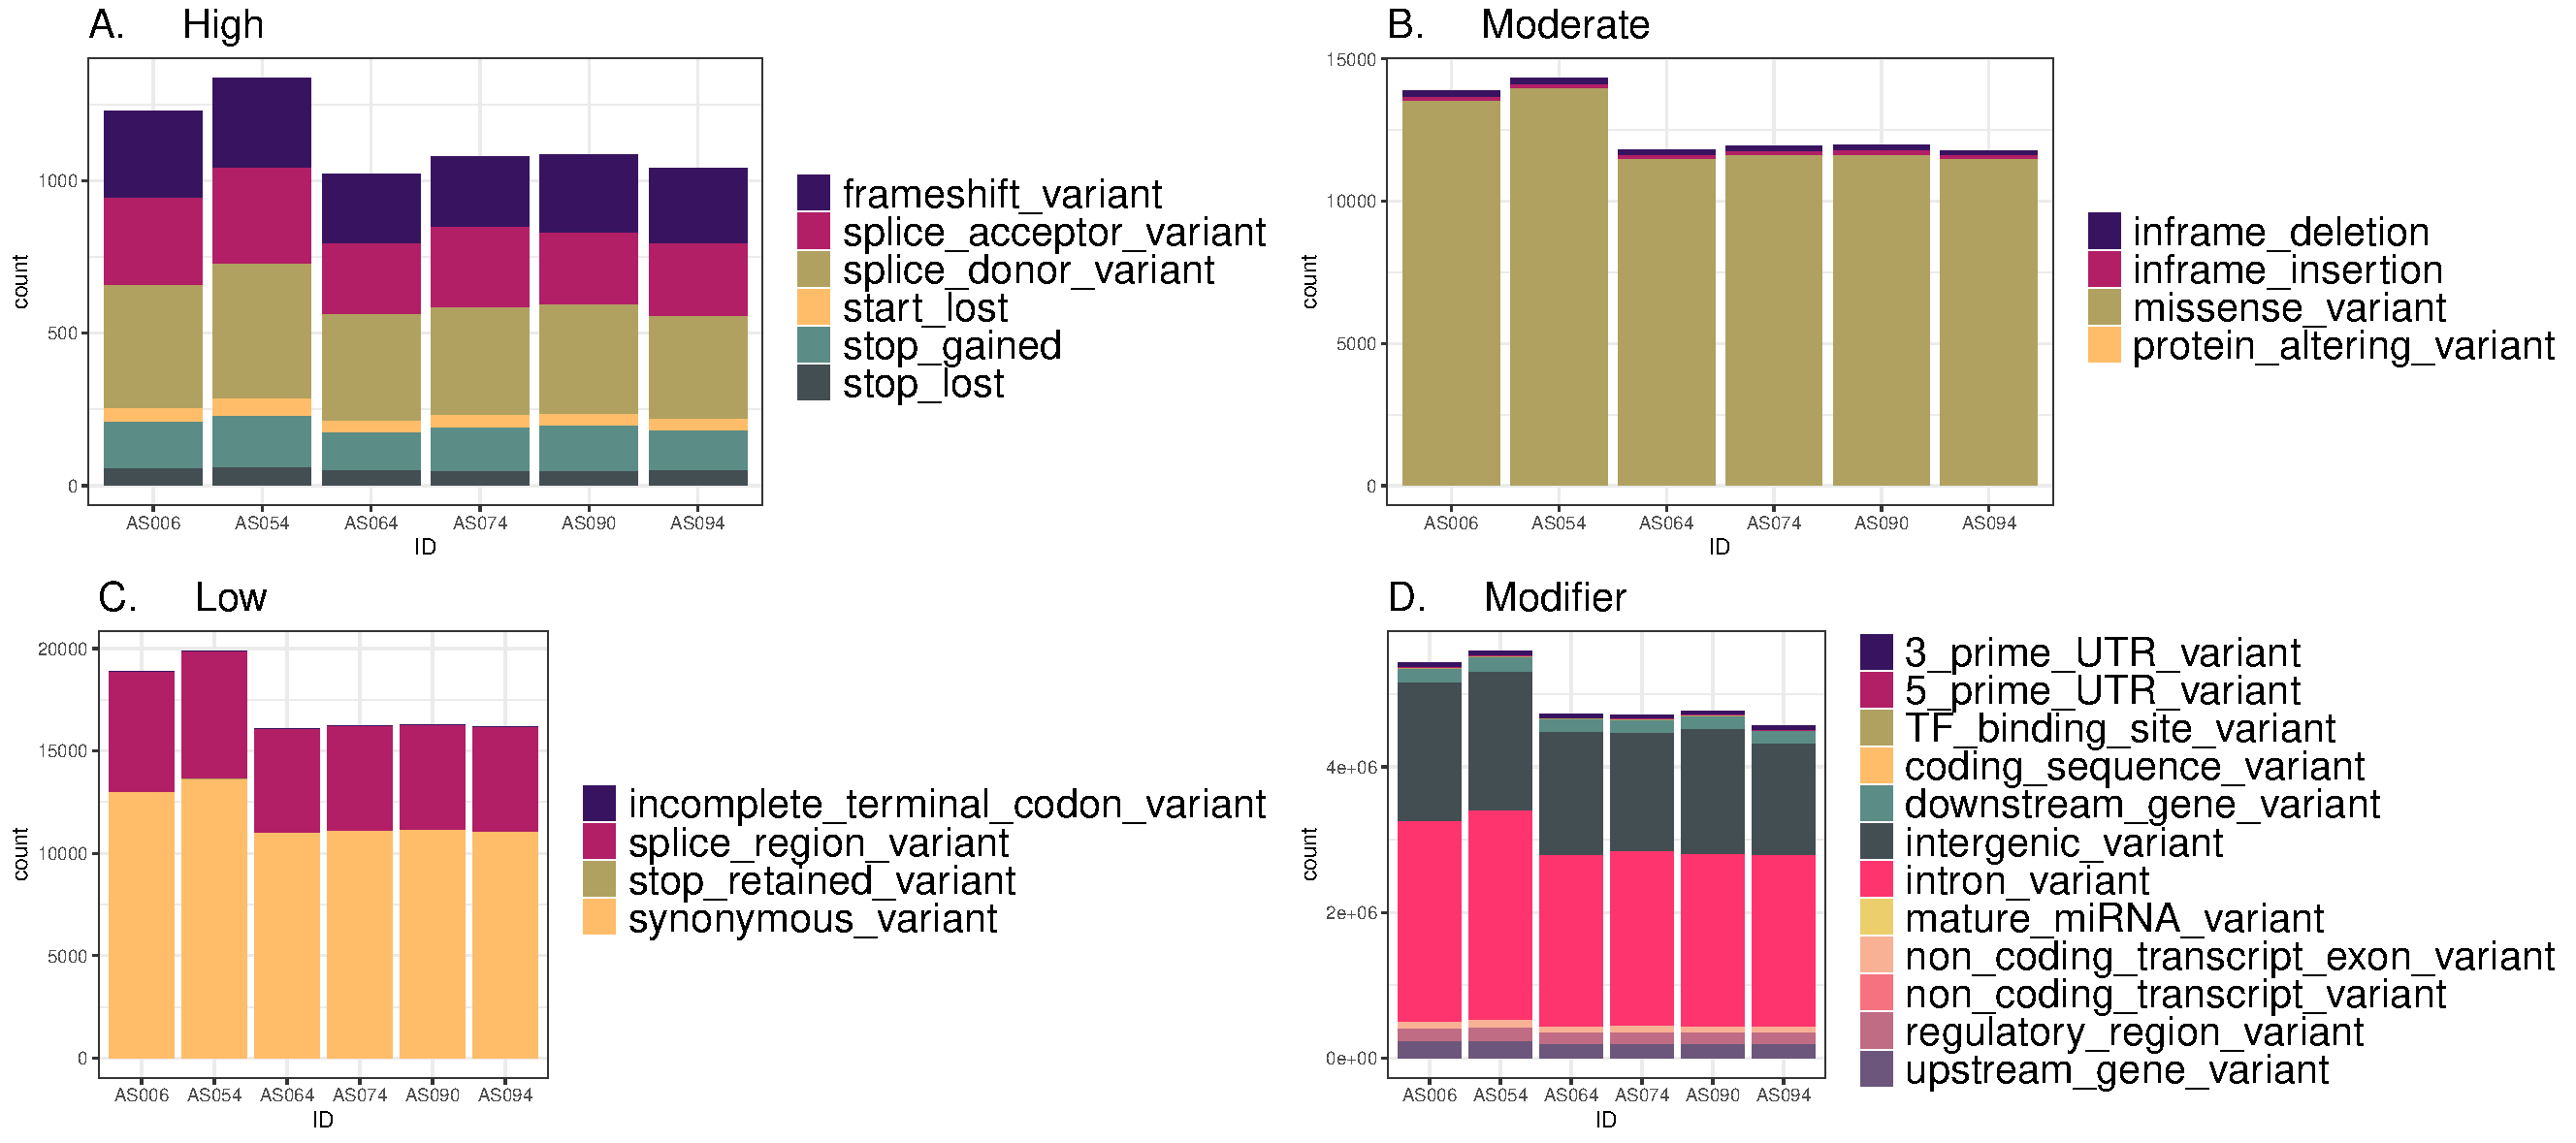
\includegraphics[width=1\textwidth]{fig/grid_cons.pdf}
\decoRule
\caption{\textbf{Functional classification of genetic variants stratified by the impact of the variant.} \textbf{Fig A High:} The most represented category is Splice donor variant, followed by Splice acceptor and frameshift variants. \textbf{Fig B Moderate:} Almost all variants with moderate impact are missense variants. \textbf{Fig C Low:} Prevalence of synonymous and splice region variants.\textbf{Fig D Modifier:} The most common categories are intron and inter-genic}
\label{fig:grid_cons}
\end{figure}


{\small
\begin{table}
\caption{Fraction variants in class of impact}
\label{tab:percentageImpact}
\centering
\begin{adjustbox}{width=0.7\textwidth}
\begin{tabular}{1 1 1 1 1 }
\toprule
\tabhead{Sample} & \tabhead{HIGH} & \tabhead{MODERATE} & \tabhead{LOW} & \tabhead{MODIFIER} \\
\midrule
 AS006 & 0.022 & 0.254 & 0.345 & 99.4 \\
 AS054 & 0.023 & 0.254 & 0.353 & 99.4 \\
 AS064 & 0.021 & 0.249 & 0.339 & 99.4 \\
 AS074 & 0.022 & 0.252 & 0.342 & 99.4 \\
 AS090 & 0.022 & 0.249 & 0.340 & 99.4 \\
 AS094 & 0.022 & 0.257 & 0.352 & 99.4 \\
\bottomrule\\
\end{tabular}
\end{adjustbox}
\end{table}
}

%%%%%%%%%%%%%%%%%%%%%%%%%%%%%%%%%%%%%%%%%%%%%%%%%%%%%%%%%%%%%%%%%%%%%%%%%%%%%%%%%%%%%%%%%%%%
%  Subsection 
%%%%%%%%%%%%%%%%%%%%%%%%%%%%%%%%%%%%%%%%%%%%%%%%%%%%%%%%%%%%%%%%%%%%%%%%%%%%%%%%%%%%%%%%%%%%
\subsection{Development of a pipeline for variant prioritization}
The rationale behind the identification of genetic variants responsible for PL is based on the hypotheses that the causative variants are likely to be among those classified as detrimental and that more than one mutation can contribute to the phenotype. Furthermore, we assume that the phenotype is a complex trait, i.e. the combination of variants at more than one gene might have caused the miscarriage, therefore we seek a list of variants in more than one gene or regulatory region, rather than a single variant. Under these assumptions, I used the information contained in the variant annotations to search for those more likely to be deleterious and possibly causative.\\

I contributed to develop a pipeline (\url{https://github.com/ezcn/grep}) that analyzes \textbf{genomic variants} within individual genome sequences to prioritize those possibly causative. A scheme of how the algorithm work is presented in Figure \ref{fig:scriptPipeline}. The pipeline is optimized for genomic regions containing coding sequences, while the analysis of regulatory regions is under development. In particular, in this first version of the pipeline we use a combination of the following information: 

%%%%%%%
\begin{figure}[H]
\centering
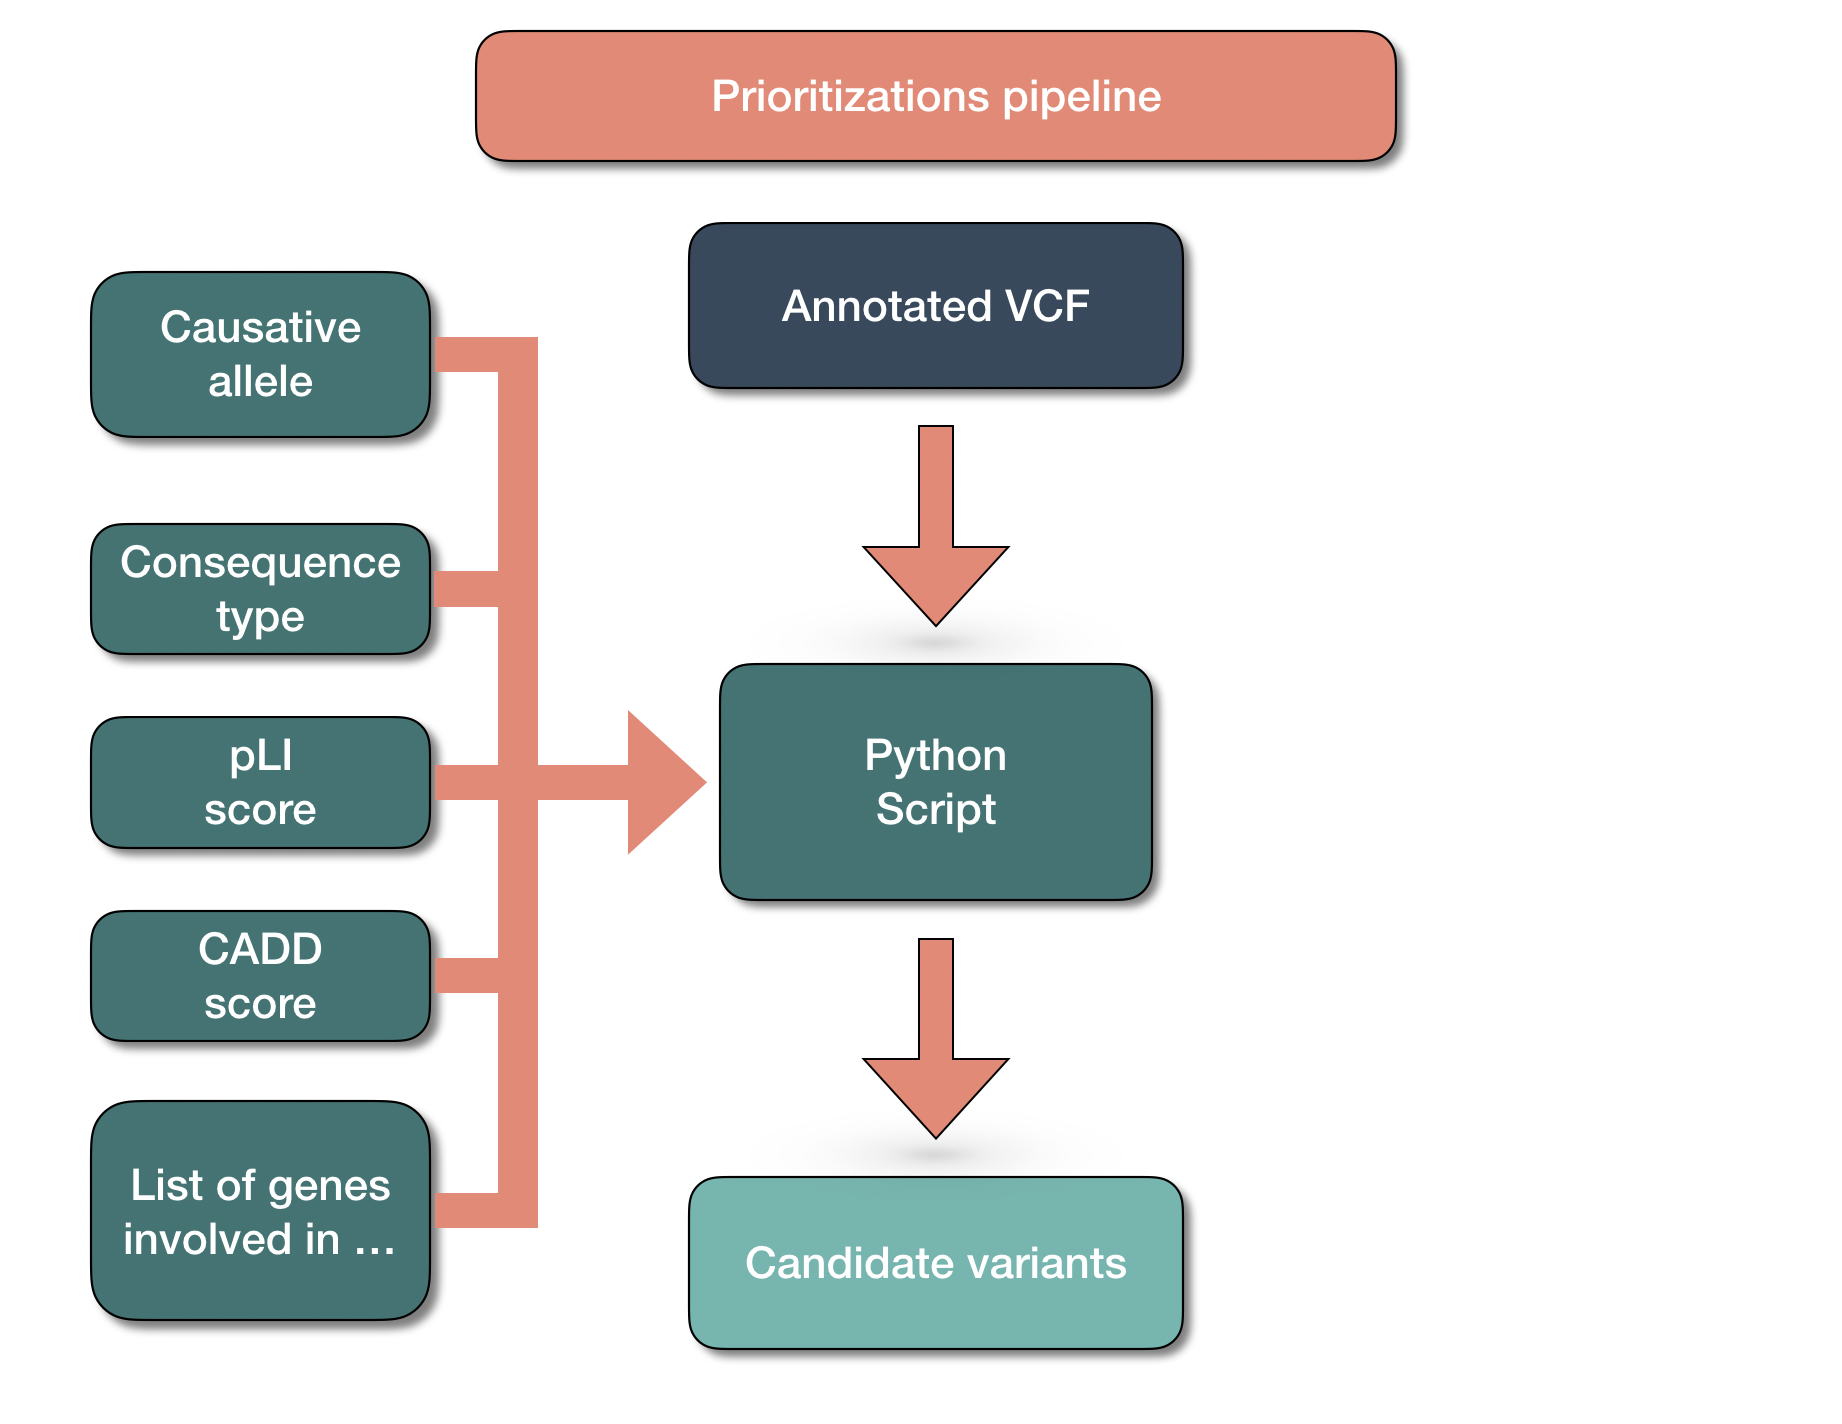
\includegraphics[width=0.85\textwidth]{fig/scriptPipeline.png}
\decoRule
\caption{\textbf{Pipeline for variant prioritization.} The pipeline combines information from variants (functional scores) and from genes to filter variants likely to be detrimental.}
\label{fig:scriptPipeline}
\end{figure}

\begin{itemize}
\item \textbf{Allele that causes the consequence.} We consider the \textbf{count} of the allele, i.e. if the individual has one or two alleles, assuming that having two alleles is worst than having only one. We consider \textbf{allele frequency} in the 1000Genomes \cite{1000genome2015global} and gnomeAD \cite{karczewskigenome} databases, representing reference population; we assume that if the allele is common than it is less likely to be detrimental. 
\item \textbf{Type and severity of the consequence.} We use the ranking illustrated in Table \ref{tab:csqVEP} to give priorities to consequences with a higher impact on the phenotype. 
\item \textbf{pLI score.} pLI is the probability of a gene of being loss-of-function intolerant \cite{lek2016analysis}. A value of pLI>0.9 suggests that the gene is likely to not tolerate mutations that alter its function, therefore variants located in these genes are more likely to be prioritized. 
\item \textbf{CADD score.} The Combined Annotation Dependent Depletion (CADD) is a score that integrates multiple annotations into one metric by contrasting variants that survived natural selection with simulated mutations \cite{kircher2014general,rentzsch2019cadd}. The highest the CADD score, the more likely is the pathogenicity of a variant and it applies both to coding and non-coding variants. 
\item \textbf{Genes associated with miscarriages or involved in embryonic development.} We assign high priority to variants located in these sets of genes: 4651 essential \cite{blomen2015gene,wang2015identification,hart2015high}; 3801 lethal \cite{dawes2019gene}; genes involved in the embryonic development (GO:0009790); 1853 genes DDD \cite{firth2011deciphering,firth2009decipher}; a manually curated list of genes that have been associated with miscarriages, obtained from literature \cite{laisk2019genetic,pereza2017systematic,qiao2016whole,rull2012genetics,colley2019potential,quintero2017novel}. 
\end{itemize}

The first part of the pipeline works at \textit{per}-individual, \textit{per}-site level producing annotations like those illustrated in Figure \ref{fig:vep_example_output}. Annotations are filtered and ranked in the second part of the pipeline. Overall, the pipeline takes as input the genetic variants in vcf format and produces a table with sites that pass the filtering or have high rank (Figure \ref{fig:scriptPipeline}). 


\begin{figure}[H]
\centering
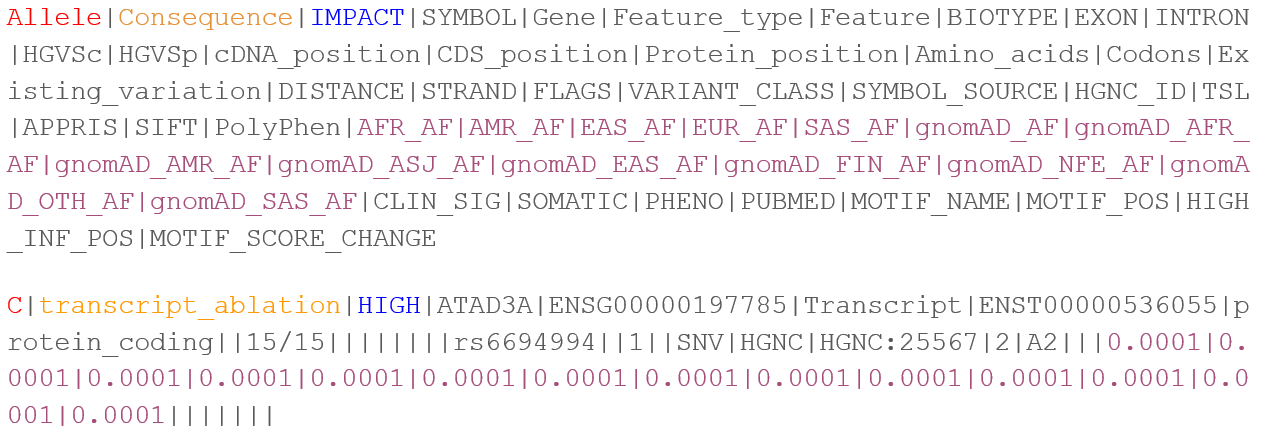
\includegraphics[width=0.9\textwidth]{fig/vep_example_output.PNG}
\decoRule
\caption[Summary Consequence]{\textbf{Header and example output of variant annotation} In the case showed here the C allele has as consequence a transcript ablation, a consequence with high impact on the gene product. This allele has allele frequency 0.0001 in all the populations considered. This is only part of the information considered in the pipeline.}
\label{fig:vep_example_output}
\end{figure}

\subsection{Identification of putatively detrimental variants by filtering and ranking of annotated variants}

\subsubsection{Filtering criteria}
Once variants are annotated, the pipeline filters variants according to different criteria. To target Rare variants with very high CADD score located in genes that are intolerant to loss of function, I used this combination of parameters: 

\begin{itemize}
\item \textbf{Impact.} Only variants with impact HIGH, MODERATE, or LOW. This criterion excludes MODIFIER variants that have a lower impact on the gene's product.
\item \textbf{Threshold for rare variants.} Only variants with frequencies <5\% in the reference populations of the 1000 Genomes and GnomeAD collections. This threshold filters for rare variants but is not too stringent to allow for causative variants to be present in the populations.
\item \textbf{Threshold for pLI score.} Only genes with pLI > 0.9. This value is typical of genes that could not tolerate mutations\cite{lek2016analysis}.
\item \textbf{Threshold for CADD score.} Only variants that have a CADD score above the 90\% percentile. This restricts to variants with highly deleterious consequences. 
\item \textbf{Consequence allele count.} Variants in heterozygosis or homozygosis.
\end{itemize}
\subsubsection{Variants retained after filtering }

When applying the filter described in the paragraph before, we identify 373 unique variants in 112 unique genes. Only one variant has high impact (stop gained), while all other variants are missense substitutions (Table \ref{tab:variatntsAfterCuration}). In each sample we identify one or more variants in 13-27 genes. Figure \ref{fig:filter2output} shows per each sample the CADD and pLI scores for the set of variants retained by the filter (yellow boxes). Notably, there are no variants in homozygosity when using this set of filters. This is expected due to the extreme values of pLI and CADD.\\

\being
{\small
\begin{table}
\caption{Number of genes per individual retained by the filter and after manual curation.}
\label{tab:variatntsAfterCuration}
\centering
\begin{adjustbox}{width=0.6\textwidth}
\begin{tabular}{1 1 1 1}
\toprule
\tabhead{Sample} & \tabhead{Variant consequence} & \tabhead{Number of genes} \\
\midrule
AS006 & missense & 24\\
AS054 & missense & 27\\
AS064 & missense & 25\\
AS074 & missense, stop gained & 23\\
AS090 & missense, stop gained & 13\\
AS094 & missense & 14\\
\bottomrule\\
\end{tabular}
\end{adjustbox}
\end{table}
}

\vspace{1,5cm}

\begin{figure}[H]
\centering
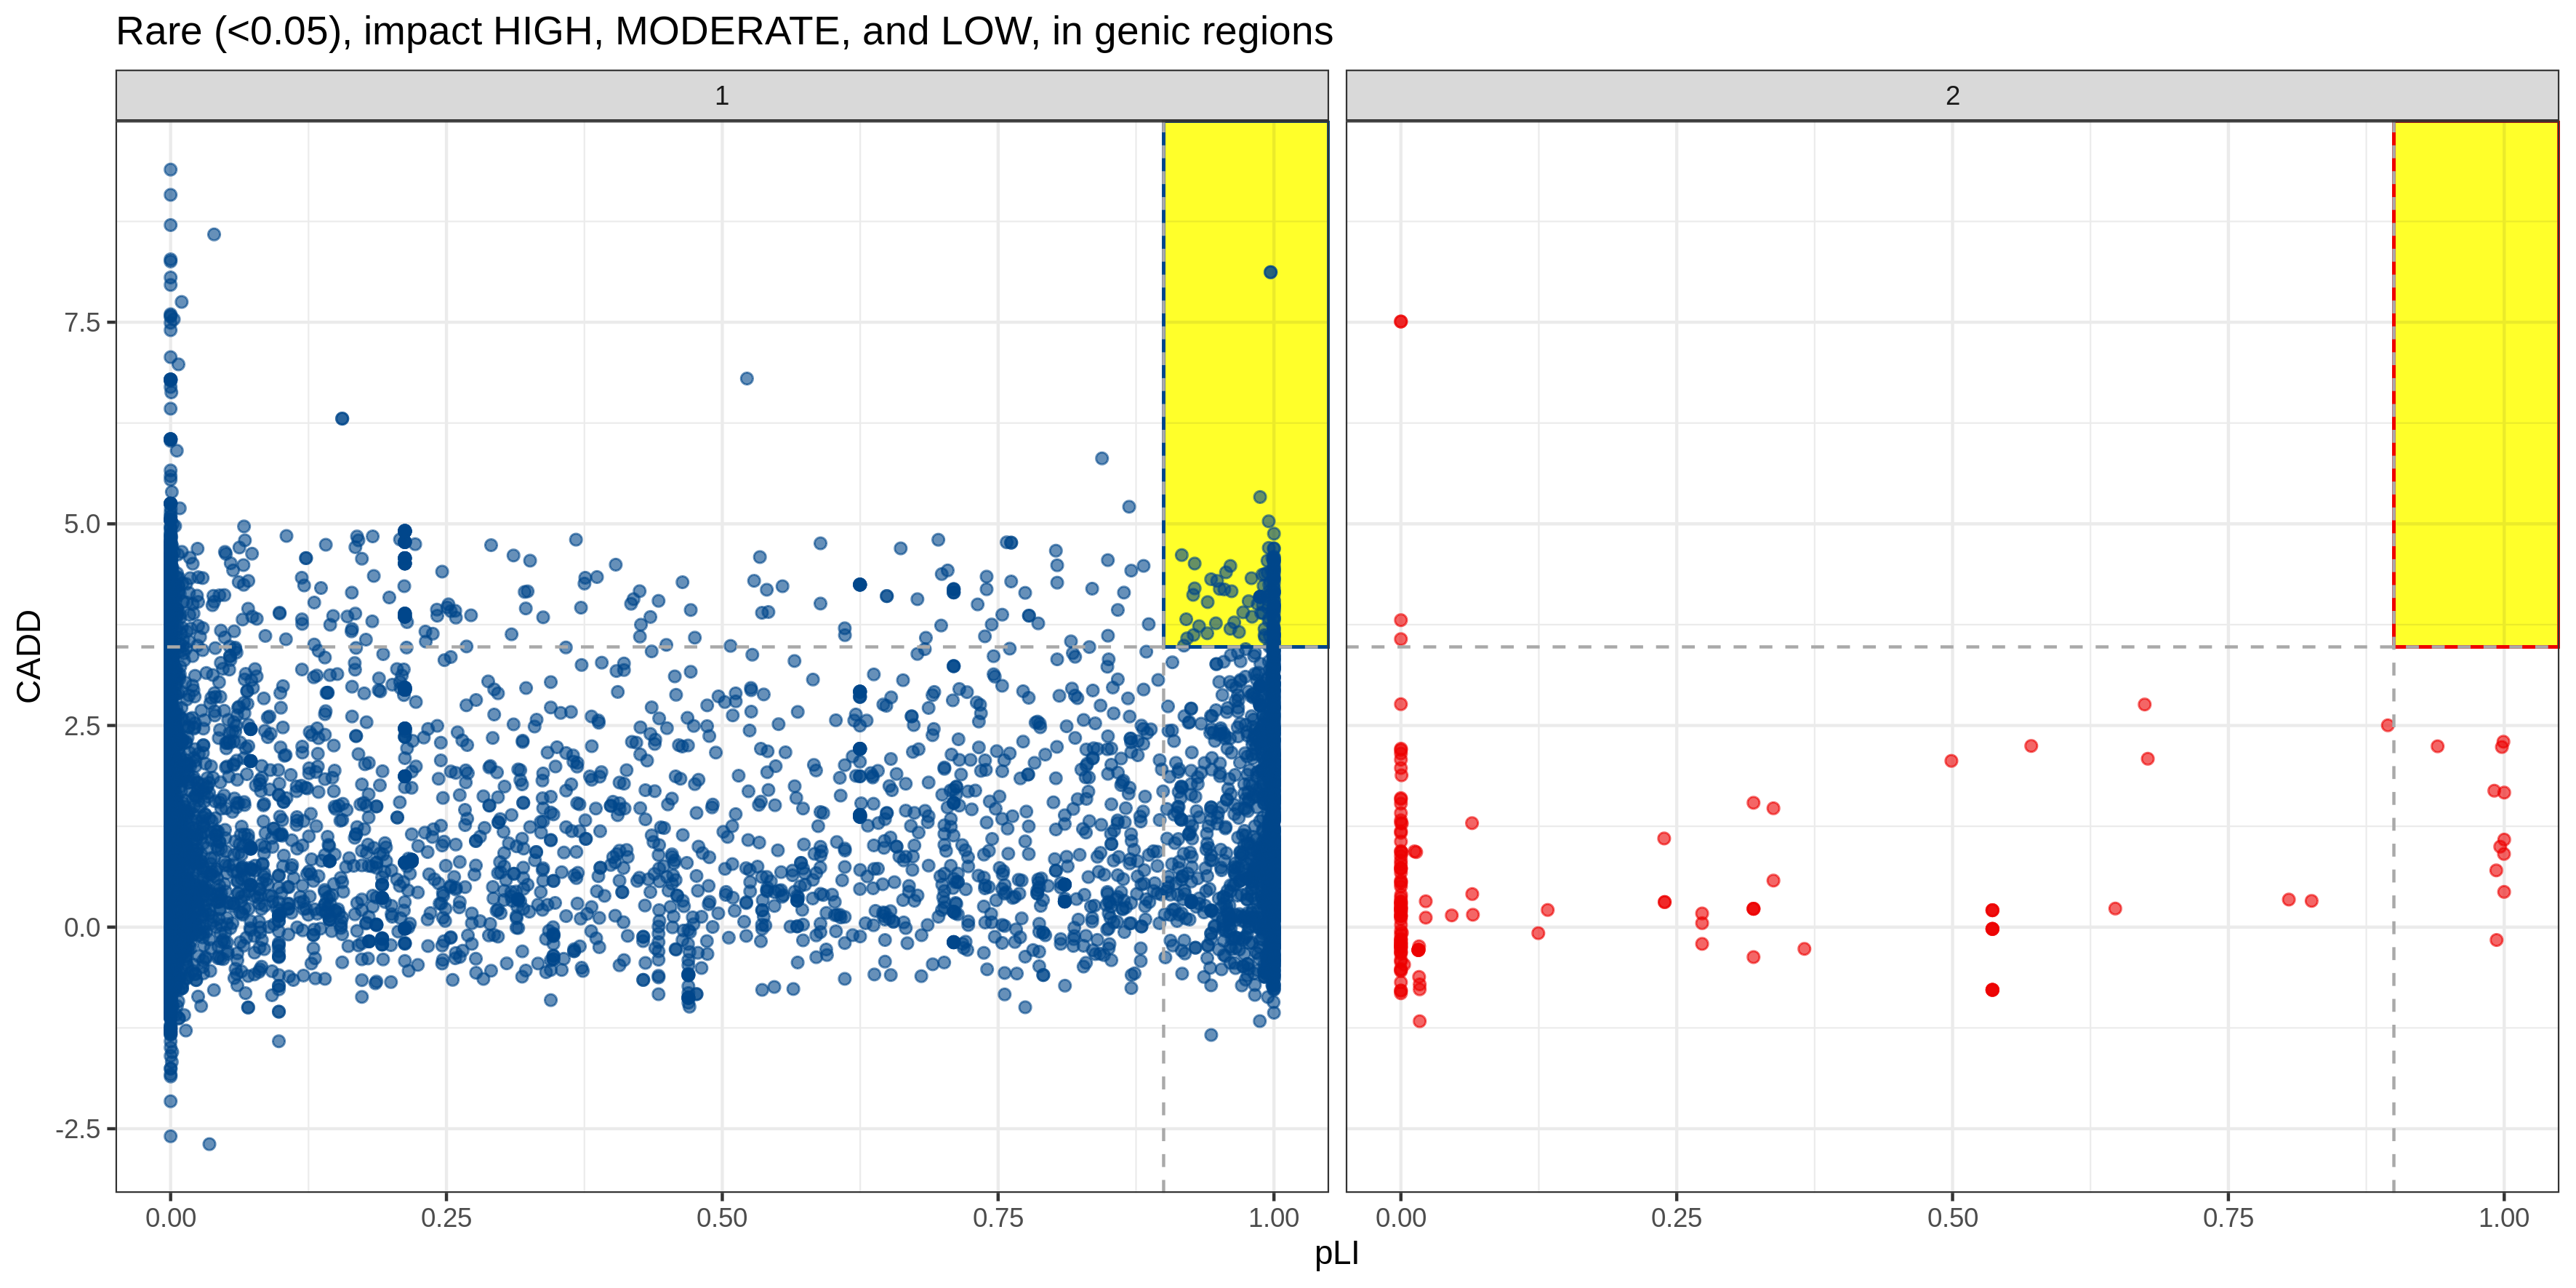
\includegraphics[width=1\textwidth]{fig/filter2py.png}
\decoRule
\caption{\textbf{Variants with high CADD and pLI.}}
\label{fig:filter2output}
\end{figure}

\subsubsection{Genes hosting filtered variants }
I aggregated the filtered variants in genes and calculated how many samples share variants in the same gene. The majority of genes are selected in only one  individual, while eleven genes are shared among two or more individuals  (Figure \ref{fig:geneCADDpLI}).\\

\vspace{1,5cm}

\begin{figure}[H]
\centering
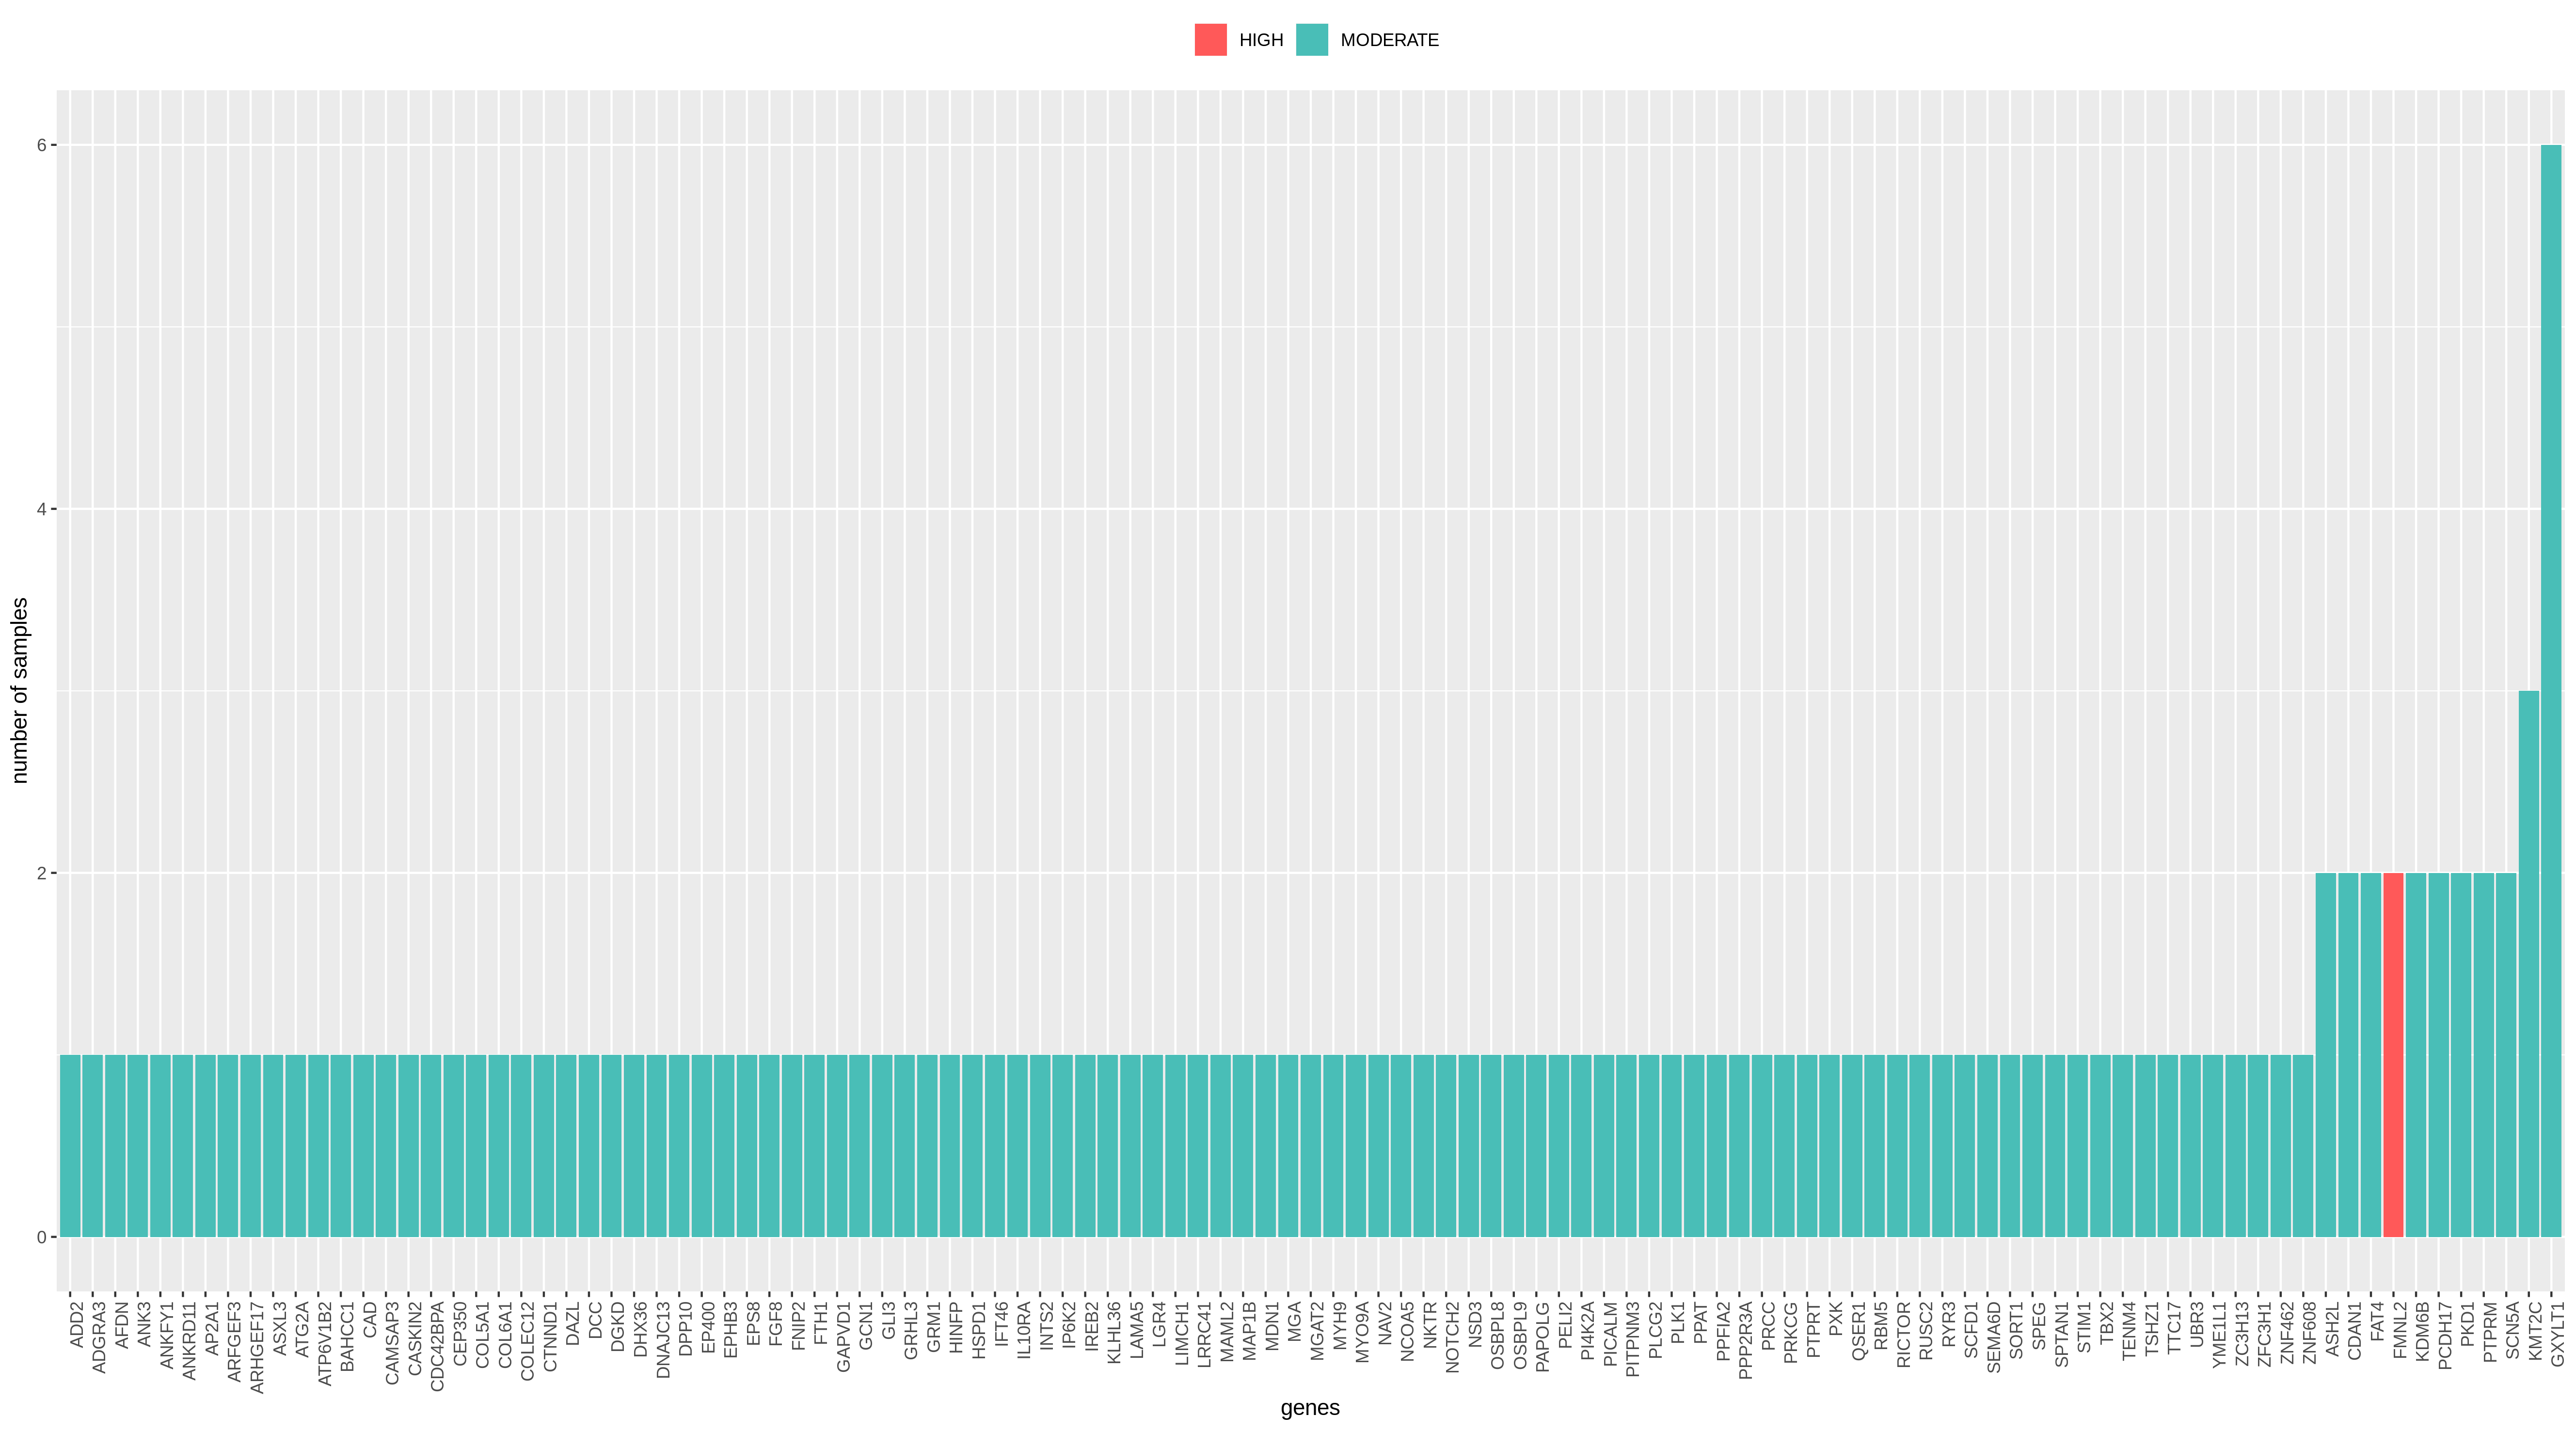
\includegraphics[width=1\textwidth]{fig/all_hetero_cadd_pli.png}
\decoRule
\caption{\textbf{Gene with high CADD and pLI.}}
\label{fig:geneCADDpLI}
\end{figure}

\vspace{1cm}

One \textbf{high impact} variant (rs750755379) that cause a Glu>Stop change in the protein is located in the sixth exon of the \textit{FMNL2} gene and is shared by two samples (Figure \ref{fig:fmnl2}). \textit{FMNL2} (ENSG00000157827) codes for a formin-related protein and has 4 transcripts (splice variants), 256 orthologues, 18 paralogues. It is located on chromosome 2:152,335,174-152,649,826 forward strand. Formin-related proteins have been implicated in morphogenesis, cytokinesis, and cell polarity. \textit{FMNL2}, in particular, is expressed in the fetus in the cytoplasm of brain, spinal cord, and rectum\cite{lizio2015gateways}. It is implicated in cytoskeleton organization (GO:0007010), regulation of cell shape (GO:0008360), cellular component organization (GO:0016043), cell migration (GO:0016477), regulation of cell morphogenesis (GO:0022604), actin cytoskeleton organization (GO:0030036), cortical actin cytoskeleton organization (GO:0030866). \\

\begin{figure}[H]
\centering
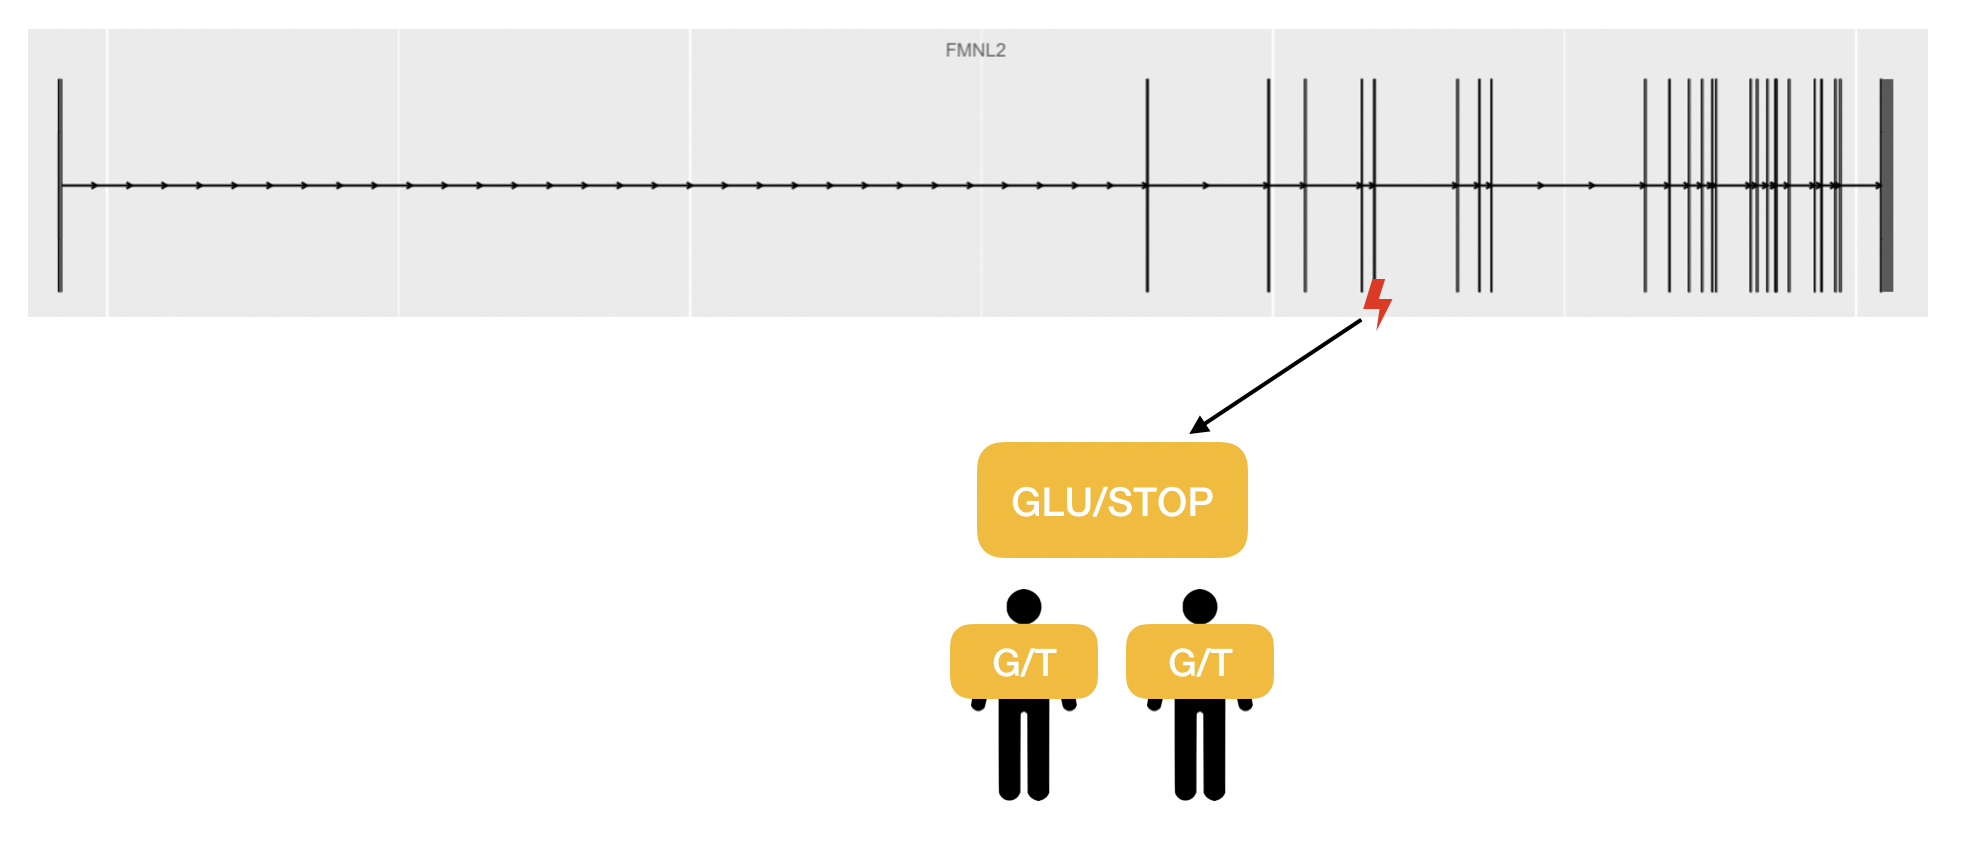
\includegraphics[width=0.95\textwidth]{fig/FMNL2_structure.png}
\decoRule
\caption{\textbf{Stop gained mutation in \textit{FMNL2} shared by two samples.} In the fetus \textit{FMNL2} is expressed cytoplasm of brain, spinal cord, and rectum where it is involved in cytoskeleton organization}
\label{fig:fmnl2}
\end{figure}

Among variants with \textbf{moderate impact}, the missense variant (rs78540738) in the fifth exone of the \textit{GXYLT1} gene is shared among all samples (Figure \ref{fig:gxylt1}). \textit{GXYLT1} is a glucoside xylosyltransferase with 2 transcripts (splice variants), 328 orthologues, 5 paralogues, located on chromosome 12: 42,081,845-42,144,874 reverse strand. The protein is a trans-membrane protein and the rs78540738 mutation corresponds to an Asp>Tyr change in the extra-cellular domain of the protein. \textit{GXYLT1} is implicated in the O-linked glycosylation\cite{sethi2010identification}, i.e. the attachment of a sugar molecule to the oxygen atom of serine (Ser) or threonine (Thr) residues in a protein.\\

\begin{figure}[H]
\centering
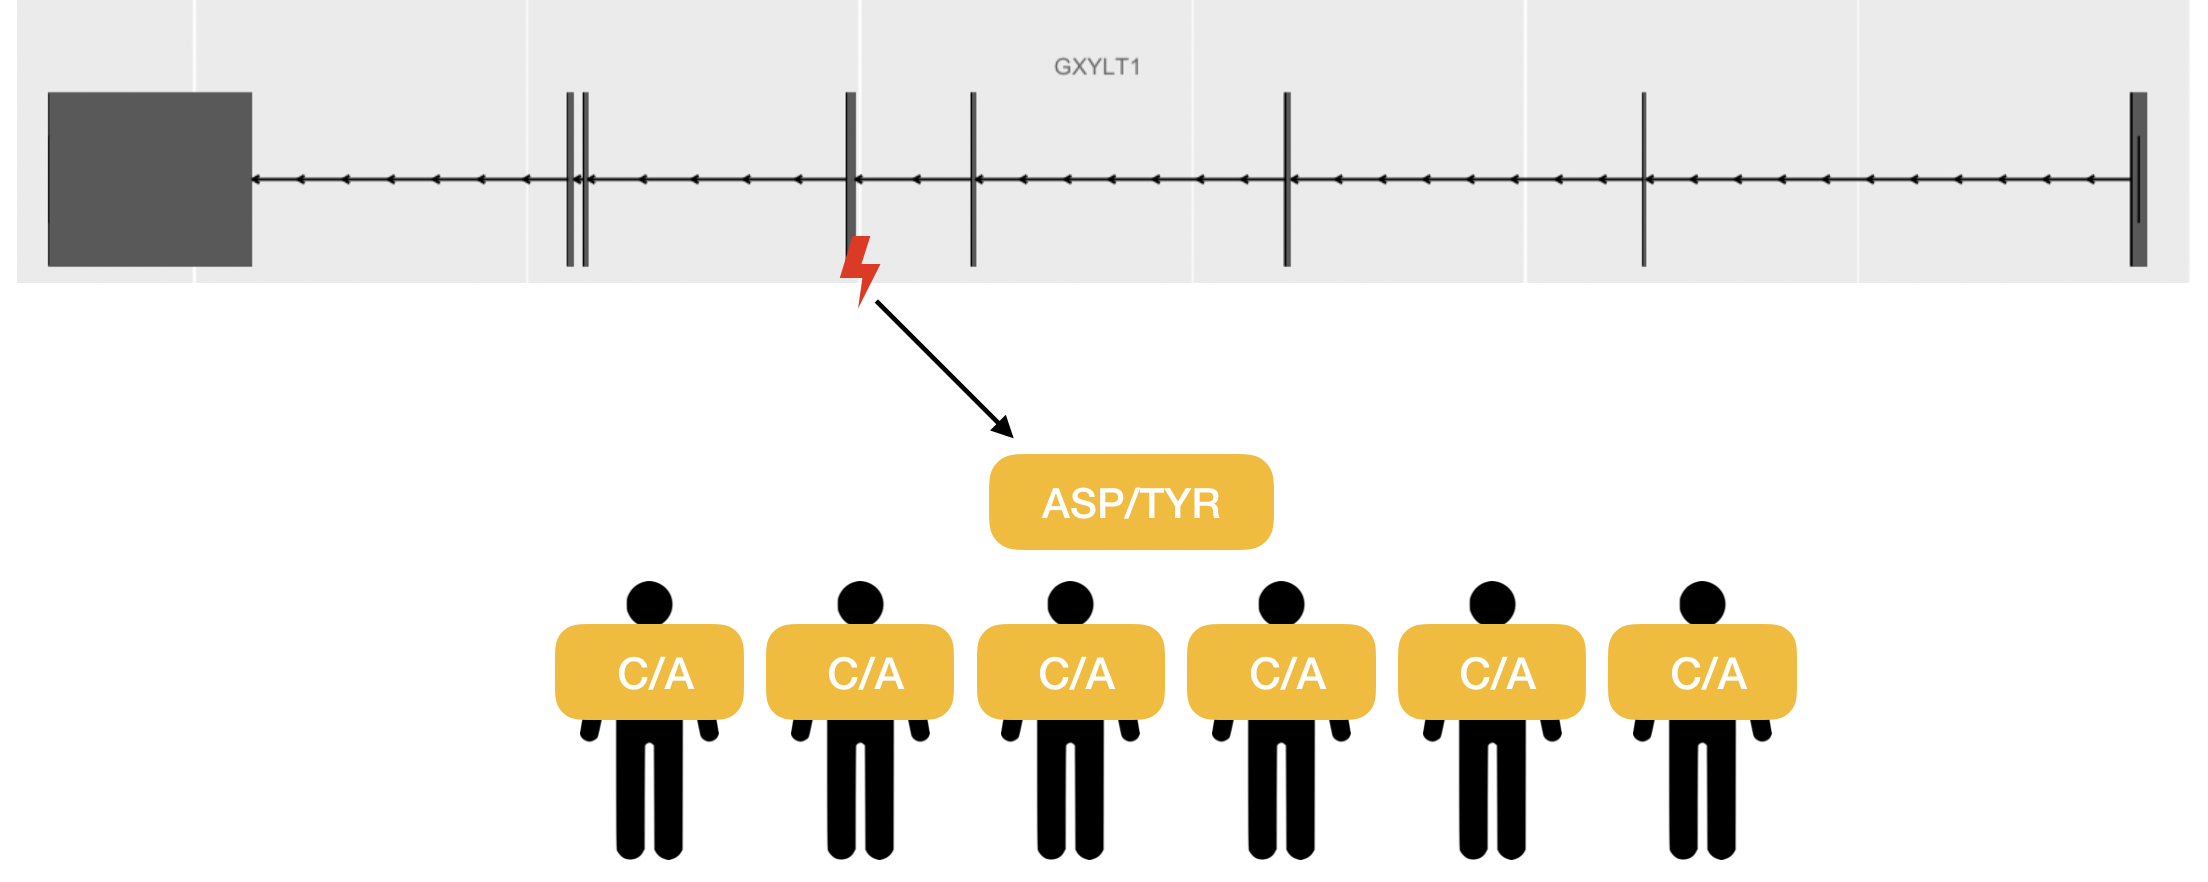
\includegraphics[width=0.95\textwidth]{fig/GXYLT1_structure.png}
\decoRule
\caption{\textbf{Missense mutation shared by all the six samples in the \textit{GXYLT1} gene.} The gene has two transcripts. The mutation we identified is rare in the general population (less than 0.01\%). \textit{GXYLT1} is a transmembrane protein. The mutation shown here corresponds  to  an  Asp>Tyr  change  in the extra-cellular domain of the protein.} 
\label{fig:gxylt1}
\end{figure}

\subsubsection{Integration of gene lists information}
To further reduce the number of genes, I integrated the information on gene lists by constraining for the variant to be in a gene that is present in at least two lists of relevant genes. The addition of this further filtering criteria, yields a list of twenty-two missense variants on average more deleterious (average CADD = 4.27) compared to previosly identified variants, located in twenty-two genes highly intolerant to loss of function (average pLI = 0.99). \\ 



%\todo{manca questa tabella, la ha silvia?}

{\small
\begin{table}
\caption{Expression level of LAMA5 in RIKEN FANTOM5 project}
\label{tab:lama5Exp}
\centering
\begin{adjustbox}{width=0.9\textwidth}
\begin{tabular}{1 1 1 1 1 1 1 1}
\toprule
\tabhead{Gene} & \tabhead{Colon} & \tabhead{Duodenum} & \tabhead{Lung} & \tabhead{Parietal lobe}  & \tabhead{Thyroid gland} & \tabhead{Umbilical cord} & \tabhead{Zone of skin}\\
\midrule
LAMA5 & 0.6 & 0.9 & 1.0 & 0.5 & 0.6 & 2.0 & 2.0 \\
\bottomrule
\end{tabular}
\end{adjustbox}
\end{table}
}

Among these genes, four samples have multiple heterozygous missense substitutions at seven sites in the \textit{LAMA5} gene (Figure \ref{fig:lama5}), located on the reverse strand of chromosome 20 in position 62,307,955-62,367,312. \textit{LAMA5} is a 59kb long gene composed of 80 exons. It has 14 transcripts (splice variants), 216 orthologues, and 28 paralogues. One of the missense mutations (rs78026347) has CADD score above the 90 percentile and cause a Pro>Leu of the 317th residue of the protein, located in a disulfide bond.
\textit{LAMA5} is a gene involved in the embryo development (GO:0009790). Mutations in \textit{LAMA5} have been associated to miscarriages \cite{laisk2019genetic,pereza2017systematic,qiao2016whole,rull2012genetics,colley2019potential,quintero2017novel} and are are lethal at early embryonic stages \cite{dawes2019gene}. It regulates the attachment, migration, and organization of cells into tissues during embryonic development. During fetal development, \textit{LAMA5} is highly expressed in the umbilical cord and in the skin (Table \ref{tab:lama5Exp})\cite{noguchi2017fantom5}.\\ 
In vertebrates, \textit{LAMA5} encodes for an alpha chain of the \textit{Laminins}\cite{aumailley2013laminin}, extracellular matrix glycoproteins composed by three non-identical multidomain chains (alpha, beta, and gamma) encoded by different genes that form a cruciform structure with one chain for each arm. \textit{Laminins} are the major noncollagenous constituent of basement membranes that are involved in cell adhesion and other different biological processes.

\begin{figure}[H]
\centering
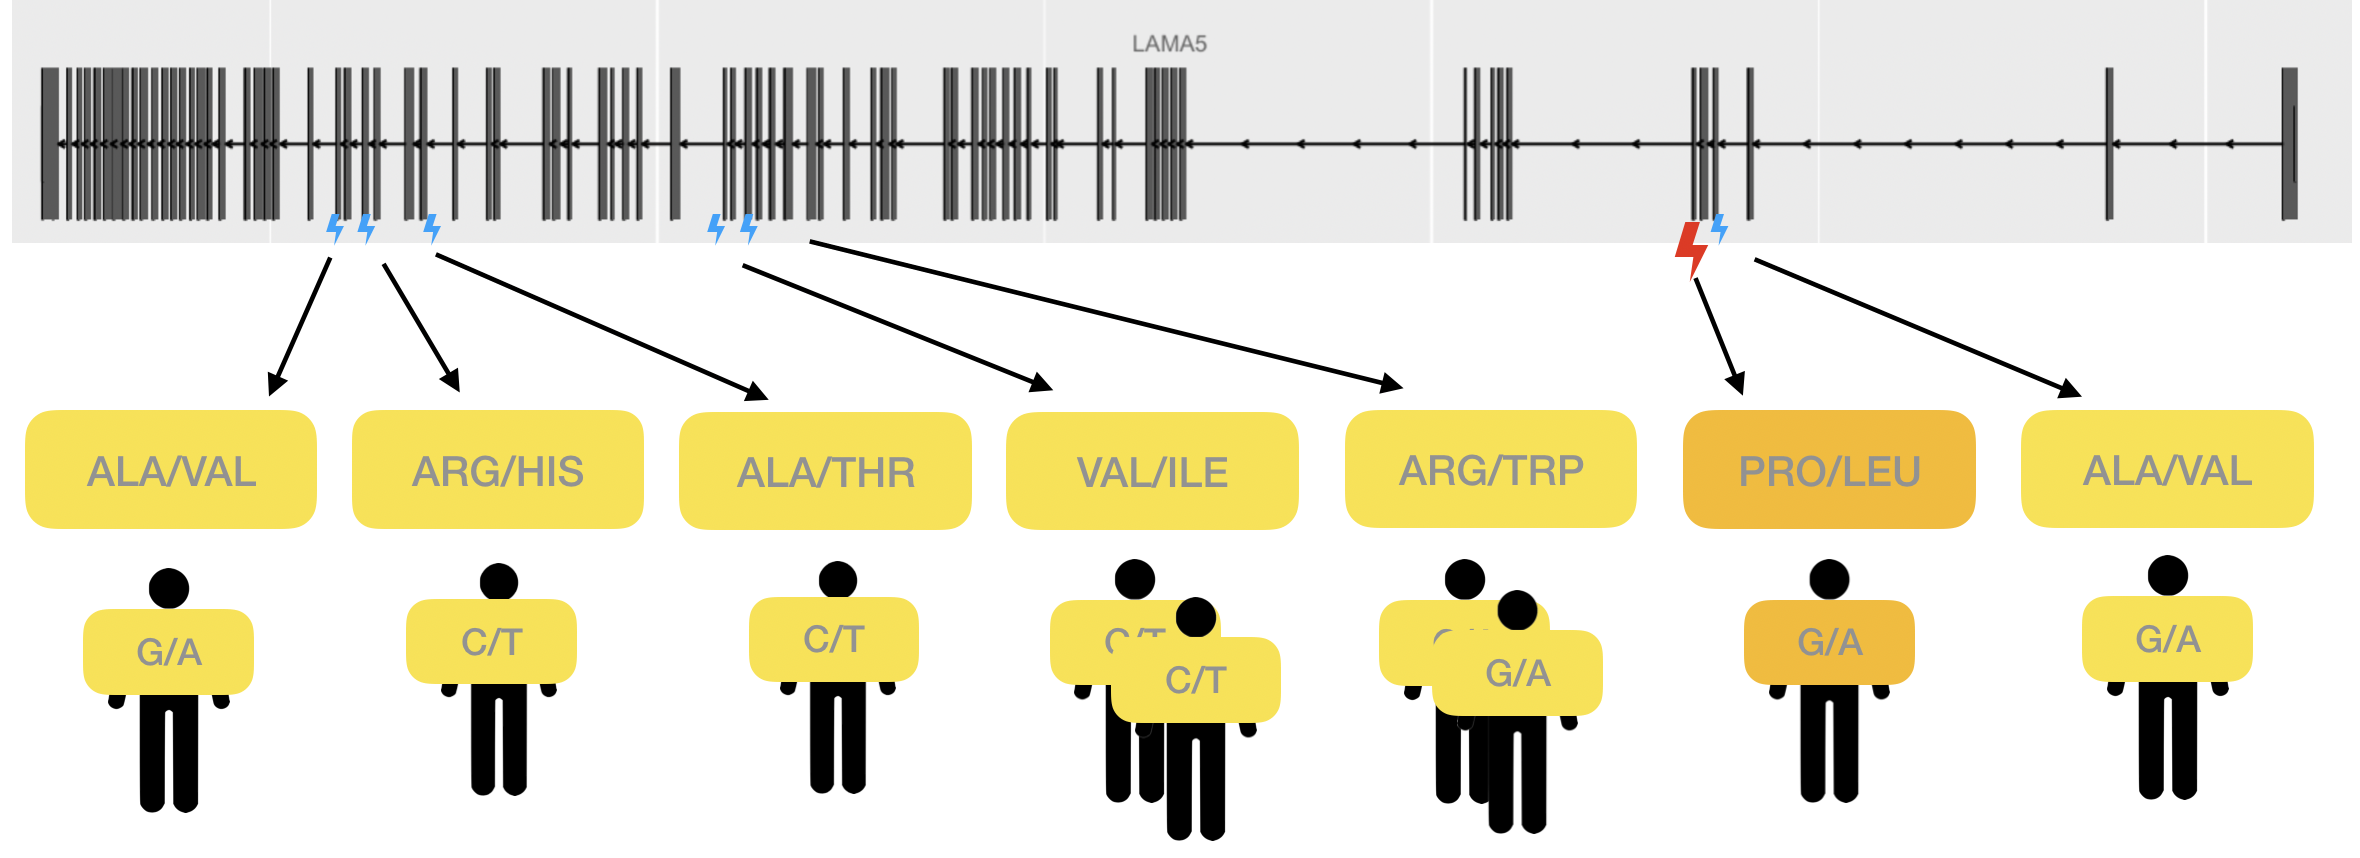
\includegraphics[width=0.95\textwidth]{fig/LAMA5_structure.png}
\decoRule
\caption{\textbf{Missense mutations in the \textit{LAMA5} gene}. \textit{LAMA5} is a gene involved in the embryo development (GO:0009790). Mutations in \textit{LAMA5} have been associated to miscarriages \cite{laisk2019genetic,pereza2017systematic,qiao2016whole,rull2012genetics,colley2019potential,quintero2017novel} and are are lethal at early embryonic stages \cite{dawes2019gene},  and in fact its pLI score is 0.94. It regulates the attachment, migration, and organization of cells into tissues during embryonic development. One of the missense mutations(dark orange) has CADD score above the 90 percentile.} 
\label{fig:lama5}
\end{figure}
